%
% Copyright (c) 2017  Pavel Kirienko <pavel.kirienko@zubax.com>
%

\documentclass{zubaxdoc}
\graphicspath{{document_templates/documentation_template_latex/}}

\usepackage{xstring}
\usepackage{multirow}
\usepackage{diagbox}
\usepackage{amsmath}
\usepackage{ConfigParamIndex}

% Draft watermark
%\usepackage{draftwatermark}
%\SetWatermarkLightness{0.85}
%\SetWatermarkText{DRAFT}

\hbadness=10000

\title{Sapog v2 Reference Manual}

\begin{document}
\frontmatter

\begin{titlepage}
\section*{Overview}

Sapog is an advanced open source sensorless PMSM\slash{}BLDC motor controller firmware designed for
use in propulsion systems of electric unmanned aircraft and watercraft.

The source repository and the public bug tracker are located at
\url{https://github.com/PX4/sapog}.

This document is applicable to firmware versions 2.x released until \today.

This document focuses only on the firmware.
Please refer to your product documentation for relevant information about the hardware.

\section*{Applications}
\begin{itemize}
    \item Propeller drives of unmanned aerial vehicles.
    \item Watercraft propulsion systems.
    \item General purpose sensorless BLDC drives.
\end{itemize}

\BeginRightColumn
\section*{Features}
\begin{itemize}
    \item Robust motor control and resilience to synchronization losses in all operating modes.
    \item Fast response. This feature is especially critical for multirotor aircraft.
    \item Regenerative braking and active freewheeling.
    \item Optional RPM control loop (RPM governor).
    \item Current limiting.
    \item Self diagnostics and extensive real-time status reporting.
    \item Compatible with most BLDC motors with very little tuning.
    \item Highly configurable.
    \item Automatic firmware update over UAVCAN in the field.
    \item Supported communication interfaces:
    \begin{itemize}
        \item UAVCAN interface with optional double redundancy.
        \item Command line interface over UART, suitable for M2M communications.
        \item RCPWM (analog PWM interface widely used in robotics).
    \end{itemize}
\end{itemize}

\end{titlepage}

\tableofcontents
\clearpage
\listoffigures
\BeginRightColumn
\listoftables

\mainmatter

\chapter{Introduction}

\section{Overview}

This document provides detailed information about the basic operating principles and
implementation details of the Sapog BLDC motor controller firmware.

This document is focused exclusively on the aspects pertaining to the firmware itself.
All questions related to particular hardware implementations are intentionally left out;
that information should be gathered from the hardware datasheets distributed by
hardware vendors.

\section{Conventions}

Unless specifically stated otherwise, all units of measurements used in this document are assumed to be SI.
Units of measurements are shown in square brackets, e.g. $\left[\text{unit}\right]$.

Within equations, references to configuration parameter values are made through the symbol $\Pi$
with the name of the configuration parameter in the subscript;
for example: $\Pi_\text{parametername}$.

\section{Definitions}

\begin{description}
    \item[PMSM] Permanent magnet synchronous motor.
    \item[BLDC] Brushless DC motor.
    \item[RPM] Revolutions per minute.
    \item[EMF] Electromotive force.
    \item[BEMF] Back electromotive force.
    \item[ADC] Analog to digital converter.
    \item[VSI] Voltage source inverter.
    \item[ESC] Electronic speed controller, synonymous to PMSM controller in the context of electric vehicles.
\end{description}

\chapter{Principles of operation}

This chapter provides a brief overview of the basic operating principles of electric permanent magnet
synchronous motors, and the relevant approaches and solutions implemented in Sapog.

\section{PMSM and BLDC motors}

\subsection{Basic equations}\label{sec:motor_equations}

This section provides the most important equations that describe a DC electric motor.
The principles explained here can be extended to all types of polyphase PMSM motors as well.

In the context of electric drives, BEMF is the voltage induced on the motor windings
while the armature of the motor is moving relative to the magnetic field of the rotor.
The induced voltage can be observed on the phase leads of the motor.
The magnitude of the induced voltage is dependent on the speed of the armature relative to the magnetic field
of the rotor, and the magnetic flux linkage of the motor. The dependency can be expressed as follows:
\begin{equation}
E_b = \phi \omega_e
\end{equation}
where $E_b$ $\left[\text{volt}\right]$ is the induced back electromotive force,
$\phi$ $\left[\text{weber}\right]$ is the magnetic flux linkage,
and $\omega_e$ $\left[\frac{\text{radian}}{\text{second}}\right]$ is the electrical angular velocity.

Electrical angular velocity is a function of the mechanical angular velocity
$\omega_m$ $\left[\frac{\text{radian}}{\text{second}}\right]$
and the number of rotor magnetic poles $N_p$:
\begin{equation}\label{eq:speed_electrical_mechanical}
\omega_e = \frac{\omega_m N_p}{2}\qquad
N_p \geq 2, N_p\text{\ is even}
\end{equation}

Both mechanical and electrical angular velocity are related to the mechanical and electrical RPM,
respectively, as follows:
\begin{equation}
\text{RPM} = \frac{30 \omega }{\pi }
\end{equation}

The armature current $I_a$ $\left[\text{ampere}\right]$ is proportional to
the voltage difference between the induced back EMF and
the source voltage $E_s$ $\left[\text{volt}\right]$:
\begin{equation}
I_a = \frac{E_s - E_b}{R}
\end{equation}
where $R$ $\left[\text{ohm}\right]$ is the internal resistance of the stator.

Torque $\tau$ $\left[\text{newton}\cdot{}\text{meter}\right]$ observed on the shaft is dependent on the
torque-generating current, flux linkage, and the number of rotor magnetic poles as follows:
\begin{equation}
\tau = \frac{\sqrt{3}}{2} I_a N_p \phi
\end{equation}

Mechanical power output $P$ $\left[\text{watt}\right]$
is the product of torque and mechanical angular velocity:
\begin{equation}
P = \tau \omega_m
\end{equation}

Motor velocity constant $K_V$ $\left[\frac{\text{RPM}_m}{\text{volt}}\right]$
is sometimes used in marketing materials and motor specifications
instead of magnetic flux linkage.\footnote{Sometimes $K_V$ is written as KV, although
this form is discouraged because it can be confused with kilovolt (kV).}
This is not a SI quantity, so its use is generally discouraged.
It can be expressed via the magnetic flux linkage $\phi$
and the number of rotor magnetic poles $N_p$ as follows:
\begin{equation}
K_V = \frac{20 \sqrt{3}}{\pi  N_p \phi }
\end{equation}

\subsection{BEMF shape}

There are two major types of permanent magnet synchronous motors (PMSM) that differ by the shape of the back
electromotive force induced while the rotor is moving at a constant speed.

The first type has a fixed magnetic flux linkage that is independent of the electrical position of the rotor.
The induced BEMF per phase therefore has a sinusoidal shape.
These motors are typically referred to simply as PMSM, or BLAC.
Since the term PMSM is quite ambiguous, we will be using the term BLAC to refer to a PMSM with sine shaped BEMF.

The other type, referred to as brushless DC, or BLDC, has a variable flux linkage that changes with the
rotor position in a specific way that results in the trapezoidal shape of the back EMF.
The difference is illustrated on the figure \ref{bemf_trapezoidal_vs_sinusoidal}.

\begin{figure}[hbt]
    \centering
	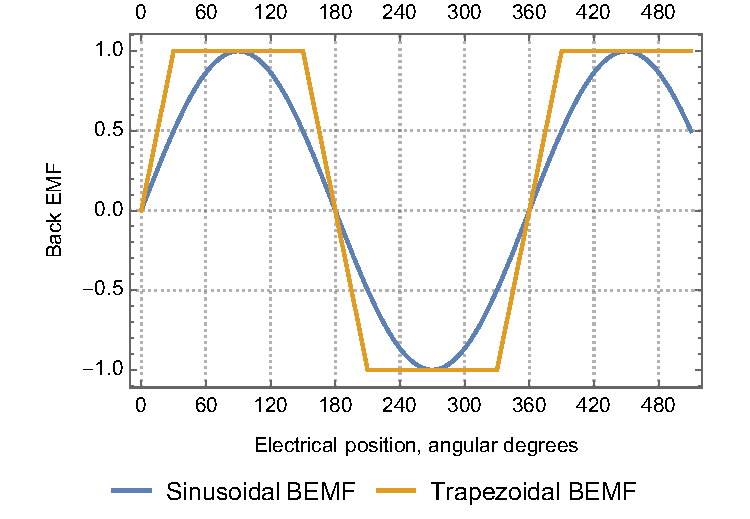
\includegraphics[width=0.6\textwidth]{bemf_trapezoidal_vs_sinusoidal}
	\caption{Difference between trapezoidal and sinusoidal BEMF.
	\label{bemf_trapezoidal_vs_sinusoidal}}
\end{figure}

Sapog, being a BLDC drive, drives the motor with trapezoidal modulated voltage.
This produces smooth torque and vibration free operation with BLDC motors,
since it is expected that the flux linkage will be changing in a specific way.

Like any BLDC drive, Sapog can operate with BLAC motors as well, albeit with increased torque ripple.
From the model presented in section \ref{sec:motor_equations} we can predict that the motor
will exhibit periodic variations in the output torque if the form of the voltage modulated by the controller
does not match with the form of the back EMF induced in the motor.
The resulting periodic torque variations that occur in a BLAC motor driven by a BLDC drive
(and, likewise, in a BLDC motor driven with sine modulated voltages) are shown on the figure 
\ref{sine_torque_deviation}.

\begin{figure}[hbt]
    \centering
	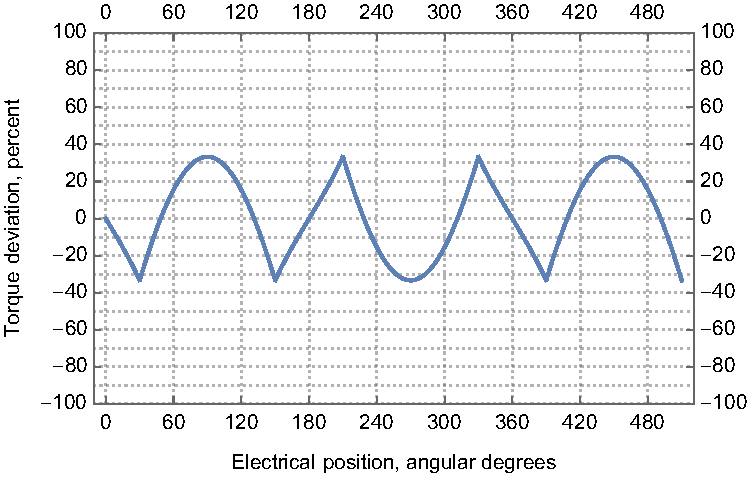
\includegraphics[width=0.6\textwidth]{sine_torque_deviation}
	\caption{Torque ripple caused by mismatching forms of the back EMF and the source voltage.
	\label{sine_torque_deviation}}
\end{figure}

Many applications, however, can tolerate the induced torque ripple and associated vibrations produced
by the motor.

\section{Motor control}

\subsection{Commutation sequence}

\newcommand{\BEMFH}{$\uparrow$}
\newcommand{\BEMFL}{$\downarrow$}

Three phase BLDC drives operate by modulating a specific sequence of voltages on the motor phases
synchronously with the movement of the rotor.
The modulated voltage sequences are shown in the commutation table below
(legend: $+$ -- positive voltage output; $-$ -- negative voltage output;
\BEMFH{} -- the phase is floating, induced BEMF is rising;
\BEMFL{} -- the phase is floating, induced BEMF is falling).

\begin{tabu}{|l c|c c c c c c|}
    \hline
    \rowfont{\bfseries}
    \multicolumn{2}{|c|}{\diagbox{Phase}{Step}}
                                 & 0     & 1     & 2     & 3     & 4     & 5     \\\hline
    \multirow{3}{*}{Forward} & A & $-$   &\BEMFH & $+$   & $+$   &\BEMFL & $-$   \\
                             & B & $+$   & $+$   &\BEMFL & $-$   & $-$   &\BEMFH \\
                             & C &\BEMFL & $-$   & $-$   &\BEMFH & $+$   & $+$   \\\hline
    \multirow{3}{*}{Reverse} & A & $-$   &\BEMFH & $+$   & $+$   &\BEMFL & $-$   \\
                             & B &\BEMFL & $-$   & $-$   &\BEMFH & $+$   & $+$   \\
                             & C & $+$   & $+$   &\BEMFL & $-$   & $-$   &\BEMFH \\\hline
\end{tabu}

The choice between forward and reverse commutation tables affects the direction of rotation of the motor,
and it is specified via the configuration parameter \CfgRef{ctl+dir}.

The rotor position is deduced from the behavior of the induced BEMF on the floating phase.
From figure \ref{bemf_trapezoidal_vs_sinusoidal} we can deduce that when the induced BEMF of the floating
phase crosses the median voltage between the high and the low phase, there is 30 electrical degrees left
before the next commutation step begins.
The controller employs this rule to estimate the time when the next commutation should occur.
The process is demonstrated on the figure \ref{commutation_basics}.
The voltage waveforms shown on the figure were acquired from the phase voltage signal conditioning circuits,
before the ADC inputs, shown on the figure \ref{power_stage_schematic}.

\begin{figure}[hbt]
    \centering
	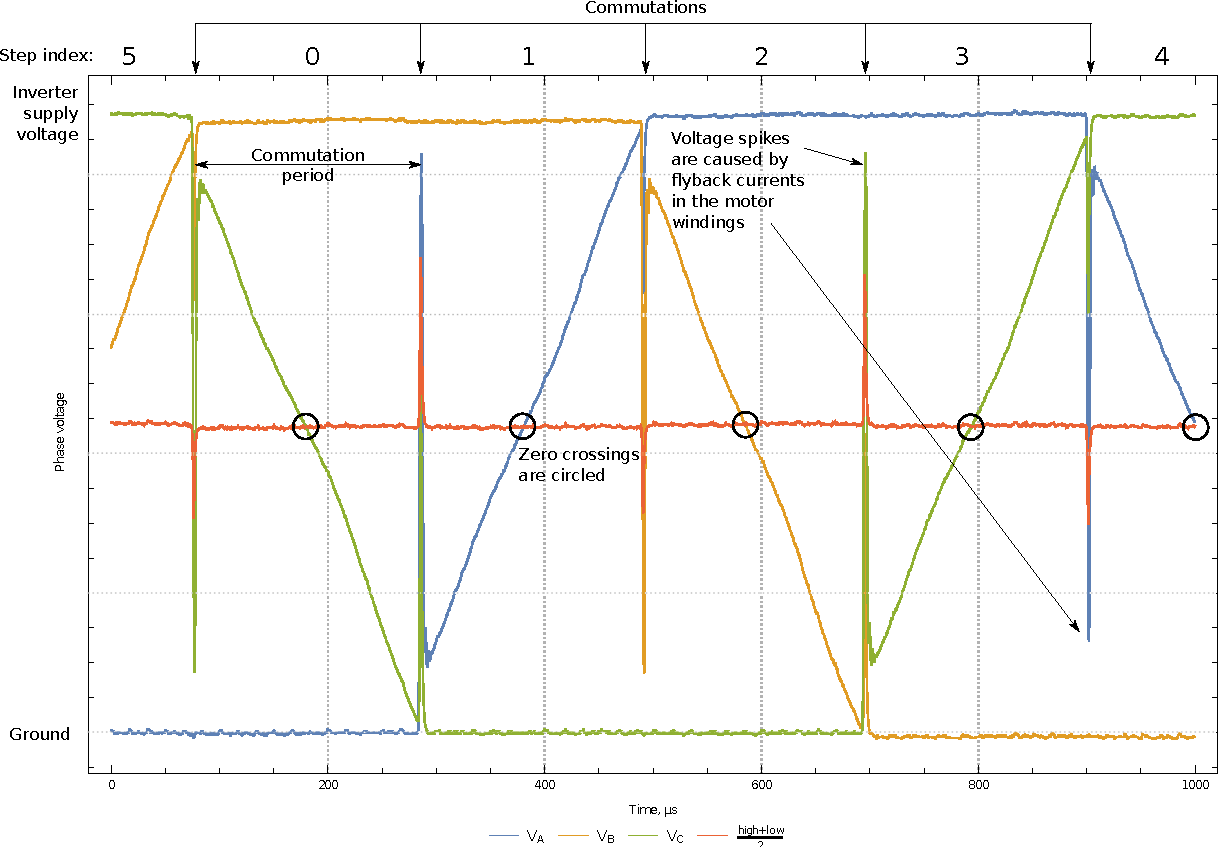
\includegraphics[width=\textwidth]{commutation_basics}
	\caption{Six step commutation sequence observed through phase voltages.
	\label{commutation_basics}}
	PWM modulation is not seen because the shown voltages were acquired while the controller
	was operating at full duty cycle.
\end{figure}

\begin{figure}[hbt]
    \centering
	
\includegraphics[width=\textwidth]{power_stage_schematic}
	\caption{Simplified schematic of the VSI and BEMF feedback circuits that Sapog relies on.
	\label{power_stage_schematic}}
\end{figure}

From the section \ref{sec:motor_equations} we know that the magnitude of the induced BEMF is linearly
dependent on the speed of relative motion between the armature and the rotor magnetic field.
Considering also the fact that the controller relies on the induced BEMF signal for rotor position estimation,
we can predict that the rotor position estimation may be unreliable if the induced BEMF is not sufficiently
strong.
In order to avoid issues at low speed operation, Sapog provides several configuration parameters that
restrict the minimum operating speed, such as the following:

\begin{itemize}
\item \CfgRef{mot+comm+per+max} - maximum commutation period, in microseconds.
The estimated commutation period will be artificially constrained to not exceed this value.
\item \CfgRef{mot+rpm+min} - minimum RPM that can be demanded in RPM governor mode.
If the demanded RPM is lower, the setpoint will be artificially increased.
Reduce this parameter to make the minimum speed lower; increase it to improve stability.
\item \CfgRef{mot+v+min} - minimum source voltage when operating in open loop mode, in volts.
If the demanded duty cycle amounts to a lower source voltage than this, the setpoint will be artificially
increased.
Reduce this parameter to make the minimum speed lower; increase it to improve stability.
\end{itemize}

These parameters may need adjustment to make Sapog compatible with a specific motor.
For example, if the motor cannot keep stable operation at low speed,
the minimum source voltage should be increased,
and/or the maximum commutation period should be made longer.
The minimum voltage limit does not apply to RPM loop mode,
where the minimum speed is governed by the dedicated configuration parameter shown above.

The following equation can be used to convert between commutation period $T_\text{comm}$
$\left[\text{second}\right]$
and electrical angular velocity $\omega_e$ $\left[\frac{\text{radian}}{\text{second}}\right]$:
\begin{equation}
\omega_e = \frac{\pi}{3 T_\text{comm}}
\end{equation}

\subsection{Source voltage modulation}

Source voltage modulation technique employed by Sapog is a fixed carrier frequency, fixed dead time,
4-quadrant, simultaneous complementary switching PWM modulation.
This modulation technique supports active freewheeling and regenerative braking.

Reviewing different modulation techniques would be outside of the scope of this document.
For more background, the reader is advised to refer to other sources, such as the article
``Influence of PWM Schemes and Commutation Methods for DC and Brushless Motors and Drives''
(Dal Y. Ohm, Richard J. Oleksuk).

The following configuration parameters govern operation of the source voltage modulator:
\begin{itemize}
\item \CfgRef{mot+pwm+hz} - PWM carrier frequency, in hertz.
\item \CfgRef{mot+pwm+dt+ns} - PWM switching dead time, in nanoseconds.
\end{itemize}

\subsubsection{PWM dead time considerations}

Generally, the end user should not change the dead time settings from the default values provided by
the vendor, because that may have unexpected negative effects on the drive.

However, in certain scenarios where a higher power output is preferred, the application may benefit from
reduced dead time intervals.
The hardware documentation may contain more useful data on this topic.

\subsection{Field weakening}\label{sec:field_weakening}

From section \ref{sec:motor_equations} we know that the maximum speed that a motor can achieve is dependent
on the the load, magnetic flux linkage, and the source voltage.
Reduction of the magnetic flux linkage decreases the induced BEMF, which allows the rotor reach higher speed,
given constant source voltage and load.

The controller can alter the commutation sequence in a specific way, causing the rotating magnetic field
created by the stator to interact with the magnetic field of the rotor in a way that reduces the magnetic
field linkage, effectively increasing the maximum speed of the rotor, reducing the output torque,
while keeping the maximum mechanical power output constant.

This technique is known as \emph{field weakening}, and it is implemented by means of adjustment of the 
commutation sequence, shortening the time interval from the zero crossing point to the moment when the next
commutation step begins.
In the context of BLDC drives this specific approach is also known as \emph{commutation advancing}.

Observe that since some part of the energy is expended on suppression of the magnetic fields induced by the
permanent magnets in the rotor, the overall efficiency of the drive decreases with stronger field weakening.

Sapog defines commutation advance angle in electrical angular degrees of rotor position,
and it can vary from 0\degree{} to 29\degree{}, inclusively, where 0\degree{} corresponds to no advance,
and 29\degree{} corresponds to the maximum advance angle.
The practical effects imposed on the drive are summarized in the following table.

\begin{ZubaxCompactTable}{|c|c c c c|}
    Advance angle & Flux linkage & Maximum torque & Maximum speed & Drive efficiency \\
    Low           & High         & High           & Low           & High             \\
    High          & Low          & Low            & High          & Low              \\
\end{ZubaxCompactTable}

Sapog can modulate a fixed advance angle, or it can be defined as a function of speed.
The latter is especially useful, since high field weakening at low speeds does not make practical sense,
and serves only to reduce the drive efficiency with no apparent benefit to the application.
Additionally, high field weakening may be responsible for stability issues at low operating speeds,
because it effectively reduces the magnitude of the BEMF induced in the motor.

The field weakening feature is configured with the help of the following configuration parameters:

\begin{itemize}
\item \CfgRef{mot+tim+adv+max} - maximum commutation advance angle, in electrical rotor position degrees.
\item \CfgRef{mot+tim+adv+min} - minimum commutation advance angle, same units.
\item \CfgRef{mot+tim+cp+min} - when the current commutation period is longer than this value,
the minimum advance angle will be used. The units are microseconds.
\item \CfgRef{mot+tim+cp+max} - when the current commutation period is shorter than this value,
the maximum advance angle will be used. Same units.
\end{itemize}

When the current commutation period is between \verb|mot_tim_cp_max| and \verb|mot_tim_cp_min|,
the advance angle will be proportionally linearly interpolated between
\verb|mot_tim_adv_min| and \verb|mot_tim_adv_max|.
The interpolation logic is demonstrated on the figure \ref{timing_advance_interpolation_plot}.

\begin{figure}[hbt]
    \centering
	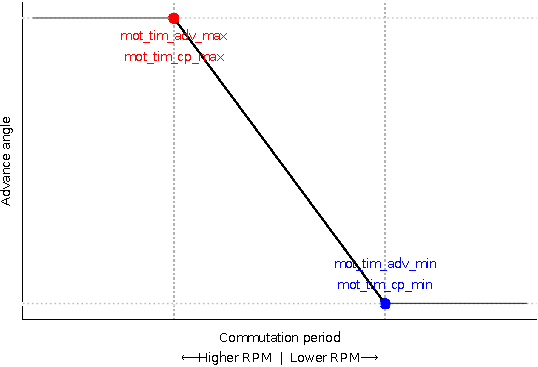
\includegraphics[width=0.7\textwidth]{timing_advance_interpolation_plot}
	\caption{Timing advance interpolation logic.
	\label{timing_advance_interpolation_plot}}
\end{figure}

Sample phase voltage waveforms acquired while the controller was operating under high field
weakening settings are shown on the figure \ref{phase_voltages_at_high_advance_angle}.

\begin{figure}[hbtp]
    \centering
	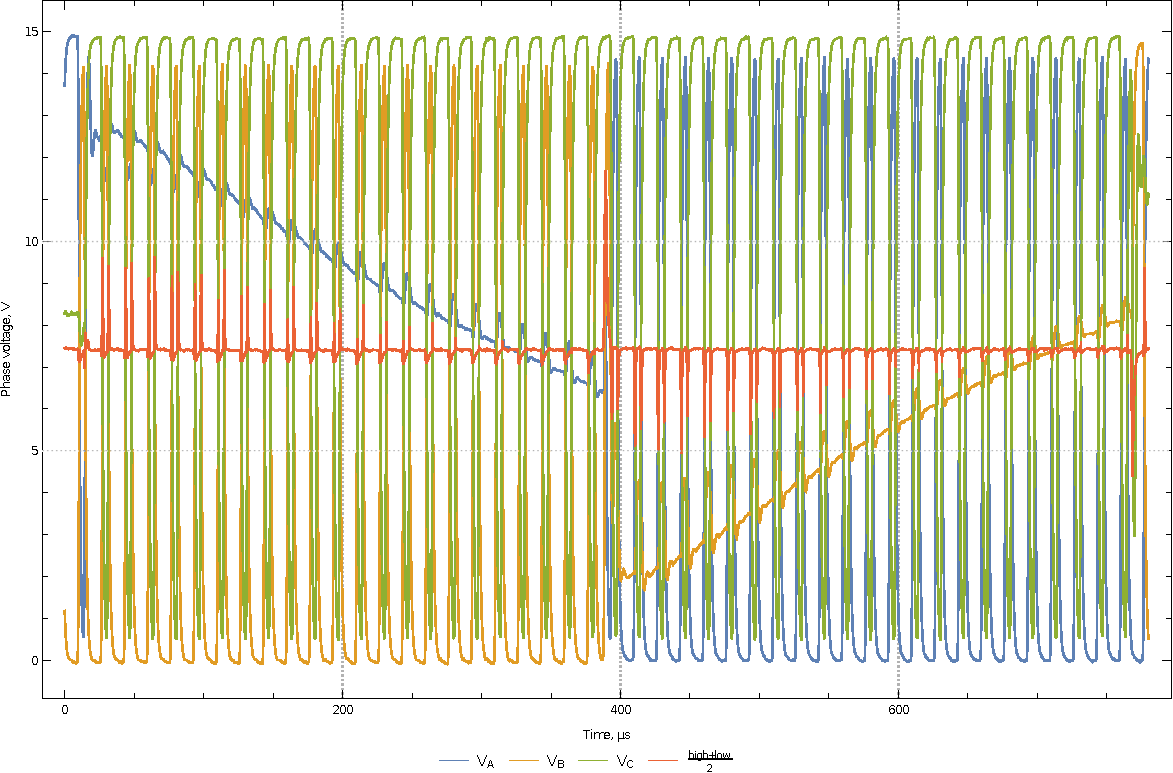
\includegraphics[width=\textwidth]{phase_voltages_at_high_advance_angle}
	\caption{Commutation sequence at high advance angle settings.
	\label{phase_voltages_at_high_advance_angle}}
	It can be seen that the next commutation begins shortly after the induced BEMF
	crosses the neutral voltage.
\end{figure}

\subsubsection{Freewheeling considerations}

Upon careful review of the field weakening effect it might become obvious that it poses a certain danger
when the motor is operating at a high speed.

According to the explanations above, as long as the field weakening is active,
the controller actively suppresses the excessive flux of the permanent magnets in the rotor.
This suppression allows the controller to lower the induced BEMF, and, therefore,
extend the operating speed upwards, while keeping the source voltage constant.

Consider what happens when the inverter (or the controller as a whole) is turned off while the
motor was running with the rotor field weakened.
As the controller ceases to suppress the field, the flux linkage of the motor returns to nominal,
which, given that the speed is sufficiently high, may significantly exceed the inverter supply
voltage $V_\text{inv}$, possibly causing damage to the controller, the power supply, the motor, etc.

\subsection{Rotor state observer}

\subsubsection{BEMF processing}

As mentioned previously, Sapog deduces the current position of the rotor by tracking the induced BEMF
on the floating phase.
Which phase is floating and the direction in which BEMF is changing is dependent on the current electrical
angle of the rotor.

Measurement of the induced BEMF is done by the ADC, which is connected to the motor phases via
resistive voltage dividers which reduce the dynamic range of the motor phase voltages into a narrower
dynamic range acceptable by the ADC,
and a buffer capacitor that provides fast recharge of the sample-and-hold capacitor of the ADC,
and suppresses high frequency noise.
The resulting simplified schematic can be seen on the figure \ref{power_stage_schematic}.

BEMF measurements are sensitive to noise. In order to avoid interference with the noise generated
by the VSI, the controller synchronizes BEMF sampling with PWM switching.
However, the timing resolution provided by the resulting sampling pattern is insufficient for robust
rotor state estimation because of the sampling period restrictions imposed by the
PWM carrier frequency.

In order to work around this limitation, Sapog collects a number of samples, and,
knowing that the shape of the BEMF induced by the floating phase of a BLDC motor is linear,
solves a linear regression problem on the collected samples, effectively recovering the most likely
shape of the BEMF signal.
The resulting approximation is very robust and resilient to noise.

The principle is illustrated on the figure \ref{phase_voltage_sampling}.

\begin{figure}[hbtp]
    \centering
	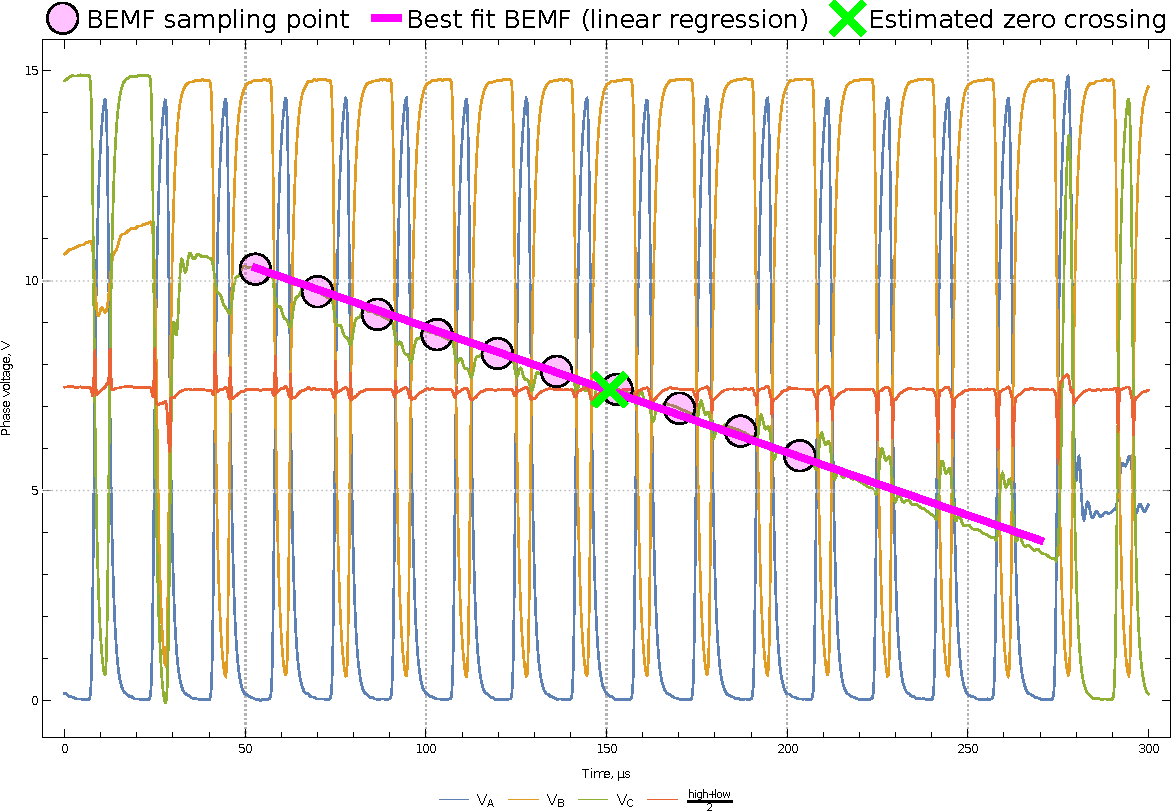
\includegraphics[width=\textwidth]{phase_voltage_sampling}
	\caption{BEMF sampling and PWM modulation.
	\label{phase_voltage_sampling}}
\end{figure}

The number of BEMF samples $N_\text{samples}$ included in the linear regression is defined by
the configuration parameter \CfgRef{mot+bemf+win+den} (dimensionless) as follows:
\begin{equation}
N_\text{samples} =
\frac{T_{\text{comm}} F_{\text{pwm}}}{\frac{\alpha\cdot{}\Pi_\text{bemfwinden}}{15} + \Pi_\text{bemfwinden}} + 2
\end{equation}
where $T_{\text{comm}}$ is the current commutation period,
$\Pi_\text{bemfwinden}$ is the value of the configuration parameter,
$\alpha$ is the current commutation advance angle in electrical rotor position degrees,
and $F_{\text{pwm}}$ $\left[\text{hertz}\right]$ is the PWM carrier frequency.

An attentive reader might point out that the assumption of linear BEMF that the described method rests
upon does not hold for BLAC motors, since the induced BEMF of a floating phase will be sinusoidal rather
than linear.
While the objection is correct, this deviation does not pose a significant problem, since the sinusoidal
BEMF well approximates to linear near the point of zero crossing.
Some issues may arise at very high advance angles, where the controller will be forced to resort to
look-ahead extrapolation, so that the linear regression will be applied to the sample set acquired
at the point where the linear approximation assumption does not hold.
The resulting imprecision, however, should not be of significant practical importance.

\subsubsection{Special cases}

The figure \ref{phase_voltage_sampling_corner_cases} provides a closer look at the challenges
seen by the controller in certain operating modes, which are reviewed below.

\begin{figure}[hbtp]
    \centering
	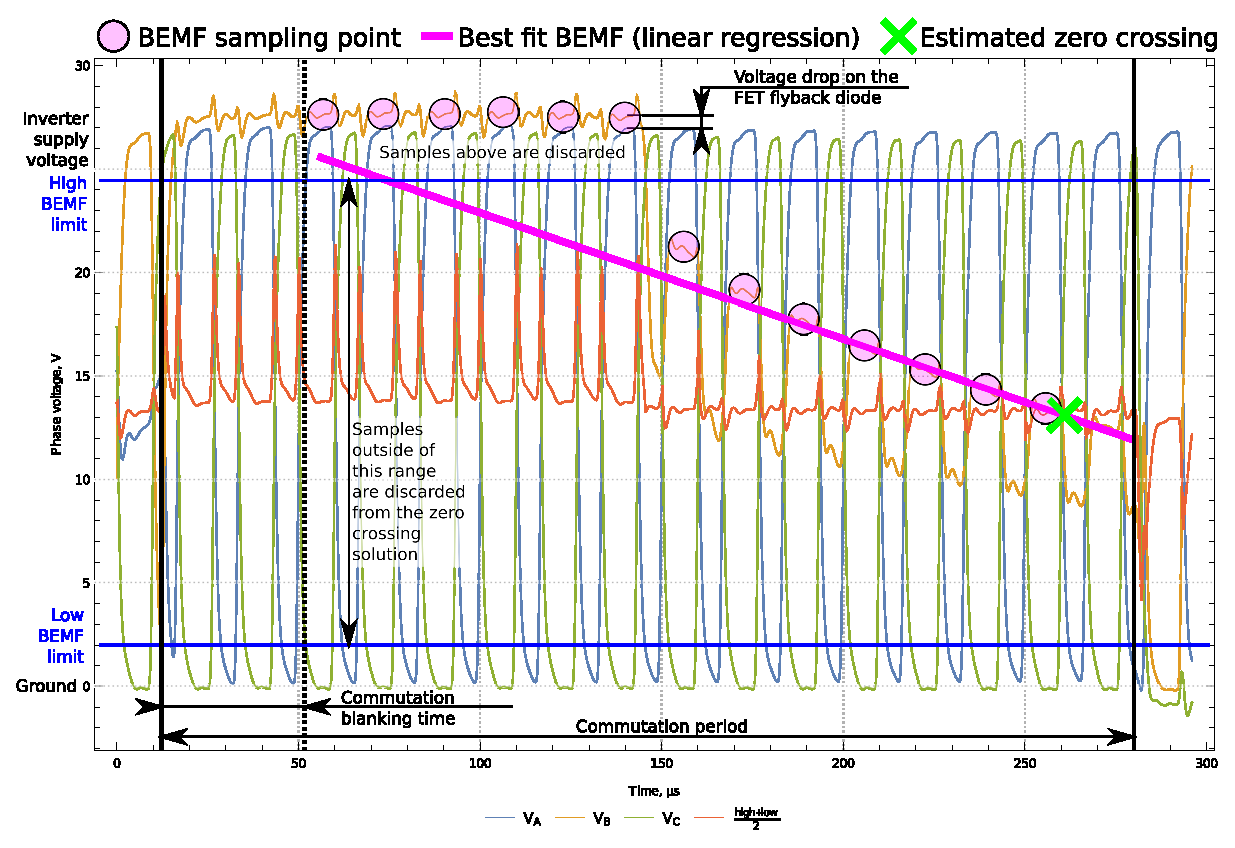
\includegraphics[width=\textwidth]{phase_voltages_braking_high_advance_angle}
	\caption{Corner cases of BEMF sampling.
	\label{phase_voltage_sampling_corner_cases}}
\end{figure}

In certain operating modes the induced BEMF of the floating phase may briefly exceed the
inverter supply voltage $V_\text{inv}$, or fall below the ground level,
causing voltage drop on either the high-side or low-side flyback diodes, respectively.
BEMF samples acquired at this time are not representative of the true form of the signal,
because the signal is altered by external factors;
and therefore, such samples cannot be used for the linear regression.
Sapog uses a simple heuristic that allows it to detect when the sampled signal is subjected to
altering and discard the affected samples.
The heuristic checks whether the sampled voltage falls into a specified range near the neutral voltage,
and discards the sample if it doesn't.

Additionally, samples acquired shortly after commutation may be subjected to transient distortions.
Sapog works around that by imposing a fixed \emph{blanking time} after a commutation, during which
BEMF sampling is not performed.

The following configuration parameters are relevant to the reviewed aspects:

\begin{itemize}
\item \CfgRef{mot+bemf+range} - the voltage range around neutral,
in percent of the inverter supply voltage $V_\text{inv}$, where the BEMF samples
will be considered valid and accepted into the solution.
\item \CfgRef{mot+blank+usec} - duration of the blanking time after the commutation, in microseconds.
\item \CfgRef{mot+spup+blnk+pm} - minimum blanking time during spin-up, permill of the commutation period.
This parameter is reviewed in more detail in a dedicated section.
\end{itemize}

Additional difficulties are posed by operation at very high power levels,
and/or when the controlled motor exhibits high inductance of the windings.
Under these conditions, the motor windings tend to accumulate significant energy during the duration
of the commutation period.
When the current commutation period ends, the winding is released, but the accumulated energy maintains
some current through the winding and the \emph{flyback diode} of one of the transistors until
the energy is dissipated.
This current caused by the energy release from a disconnected inductive network is known as
\emph{flyback current}.
As long as the flyback current is flowing though the winding and the flyback diode,
the induced BEMF is completely suppressed and, therefore,
is unobservable, which does not allow the controller to evaluate the state of the rotor.

\begin{figure}[hbtp]
    \centering
	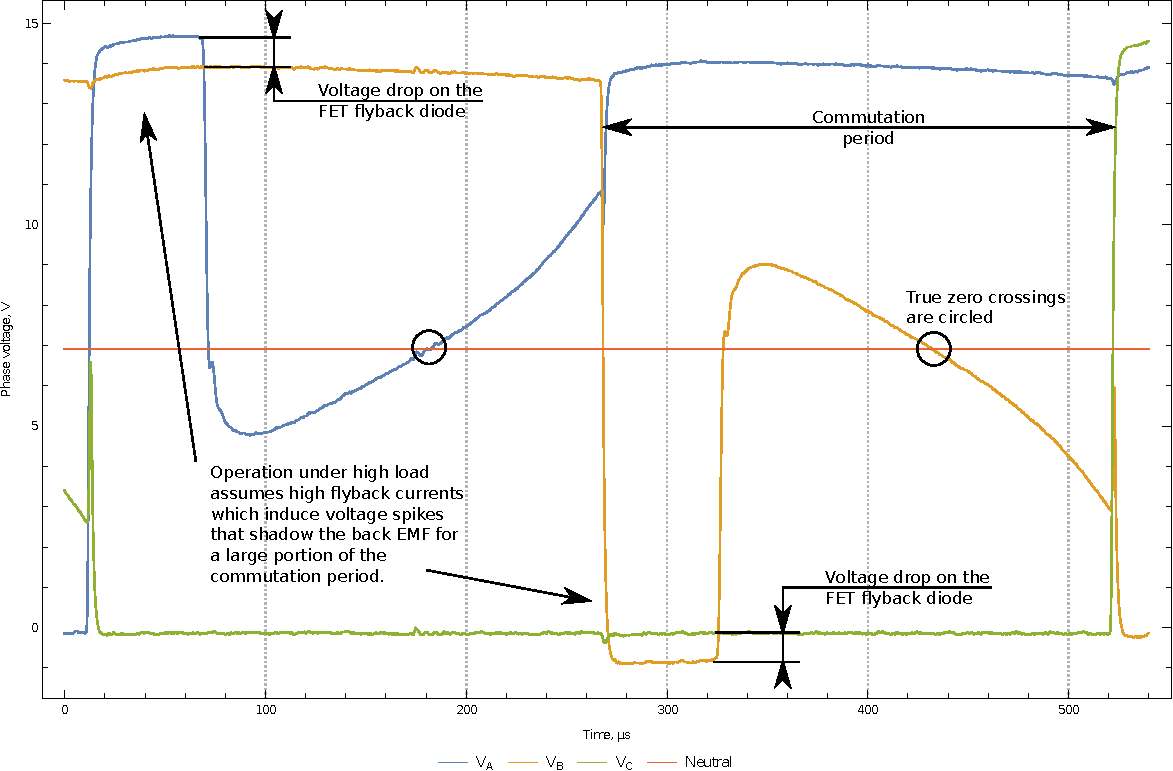
\includegraphics[width=\textwidth]{phase_voltages_at_high_load}
	\caption{Challenges of high power operation.
	\label{phase_voltages_at_high_load}}
\end{figure}

Sapog recognizes this condition and waits for the flyback current to cease.
If the current is still flowing past a certain deadline necessary for the controller to evaluate the
point of zero crossing, Sapog enters a \emph{desaturation mode} in order to bring the system
back into observable state.
In the desaturation mode Sapog turns off the inverter and waits until the next commutation period.
By the time the next commutation period begins, the flyback currents will have ended,
allowing the controller to continue observation of the motor state.

The figure \ref{phase_voltages_at_high_load} shows operation near the point of activation
of the desaturation mode.

\subsubsection{Maximum speed restrictions}

It is easy to see that as the speed increases and the commutation period shortens,
the number of BEMF samples that can be accommodated within the commutation period will be decreasing.
This effect imposes the limit on the maximum achievable speed, and the limit is dependent on the PWM
carrier frequency.

When the drive operates in open loop mode, the controller will limit the maximum duty cycle
when the commutation period reaches dangerously low values.
The limiting is done by means of a simple P-controller,
which begins to override the duty cycle setpoint when it exceeds a certain value.

When the drive operates in RPM control loop mode, the limiting will be performed simply by means of
clipping the RPM setpoint.

The exact thresholds are specified on the figure \ref{pwm_maximum_speed}.

The configuration parameter \CfgRef{mot+pwm+hz} can be used to set the desirable PWM frequency
in hertz.
It is recommended to keep the frequency as low as possible,
as that would facilitate lower switching losses and therefore higher efficiency of the drive.

\begin{figure}[hbt]
    \centering
	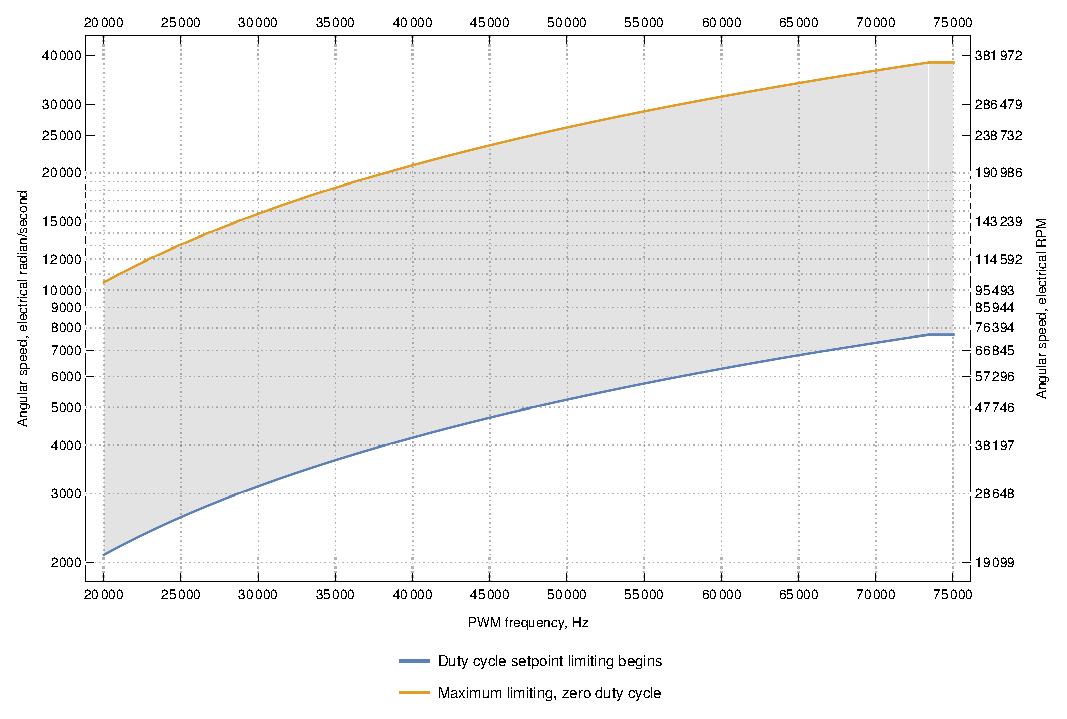
\includegraphics[width=\textwidth]{pwm_maximum_speed}
	\caption{Dependency of the maximum speed on PWM frequency.
	\label{pwm_maximum_speed}}
\end{figure}

\subsubsection{Field weakening restrictions}

The controller requires several microseconds to solve the linear regression problem after the sampling is
finished.
However, operation at very high advance angles requires the controller to perform commutation virtually
immediately after the zero crossing has happened, leaving very little time to perform the computation.
The controller strives to work around this contradiction by trying to robustly extrapolate the shape of the
BEMF signal, predicting the upcoming zero crossing ahead of time.

Despite that, operation at very high speeds may not provide the time necessary to take a sufficient
number of samples and solve the regression problem before the next commutation is due.
In this case, Sapog will silently lower the current advance angle and keep it at as close to the requested
value as the current operating mode permits.

\subsection{Regenerative braking}

During regenerative braking, the source voltage $E_s$ modulated by the controller is lower than the
induced BEMF $E_b$, which causes reverse current flow from the motor into the VSI
and further into the power supply network.
According to the formulas presented in the section \ref{sec:motor_equations},
reversing the current will also reverse the torque, causing the motor to rapidly decelerate.

This process converts the mechanical energy of the motor into electrical energy returned back into the
power supply network.
If the power supply network cannot absorb the recovered energy (e.g. due to its resistance being too high),
the regenerative energy transfer may lead to increase of the supply voltage beyond the safe operating limits.
Typically, the controller hardware is equipped with some protection circuits that activate and dissipate the
excessive energy when $V_\text{inv}$ increases a certain threshold;
however, their energy absorption capabilities are often very  limited.

Generally, batteries are capable of absorbing the regenerated energy during braking without issues.
Problems may arise if the controller is powered from a source that does not permit reverse currents,
such as laboratory power supplies or some types of voltage conversion circuits.

Refer to the documentation provided with your hardware to learn more about the issues
concerning regenerative braking and the excess energy release.

\subsection{Rotor stall detection}\label{sec:stall_detection}

Rotor stall is a condition where the rotor ceases to rotate due to the torque generated by the motor
being lower than the mechanical load on the shaft.
Sapog detects this condition by observing a specific number of failures to find
a valid BEMF zero crossing event.

As explained in one of the earlier sections of this document,
Sapog requires the rotor to move in order to be able to operate normally.
Once the rotor has stalled, Sapog will shut down the VSI and wait for the next setpoint to arrive.
Once the next setpoint has arrived, Sapog will restart the motor normally,
unless the number of consecutive stalls has exceeded a specific limit.

In the latter case, Sapog will lock up and refuse to start the motor again,
until it has received a zero setpoint.
Zero setpoint is treated as a reset command that clears the stall counter and unlocks the controller.

Zero cross failures are counted with the help of a dedicated counter state.
When Sapog fails to find a zero crossing solution,
the failure counter is incremented by one.
When Sapog succeeds to perform six (6) commutations in a row without failures,
the failure counter is reset back to zero.

The following configuration parameters configure the behaviors pertaining to stall detection:

\begin{itemize}
\item \CfgRef{mot+zc+fails+max} - zero crossing detection failure threshold.
If the failure counter exceeds this threshold, the rotor will be considered stalled.
\item \CfgRef{mot+stop+thres} - lock-up threshold.
If the rotor has stalled this number of times in a row,
the controller will lock up until a zero setpoint is received.
\end{itemize}

\subsection{Spin-up}

As has been explained before, Sapog requires the rotor to move in order to be able to operate normally,
because the state estimation methods that work well when the rotor is moving break apart when the rotor is
stationary or nearly so.

From the above follows that a different method of state estimation is needed to start the motor
from standstill, especially so if the shaft is attached to a mechanical/inertial load.

\subsubsection{Algorithm}

When starting the motor, Sapog sets the source voltage $E_s$ to the value specified in the
configuration parameter \CfgRef{mot+v+spinup}, and activates the commutation step at the index 1.
Having done so, Sapog begins to wait for the zero crossing detector to report that it is time to
begin the next commutation period, or until the amount of time specified by the configuration parameter
\CfgRef{mot+spup+st+cp} expires, whichever happens first.
Afterwards, Sapog switches to the next commutation step, and the process repeats again.

While in spin-up mode, Sapog will slowly increase the voltage from the initial value specified
by \CfgRef{mot+v+spinup} until the minimal operating voltage \CfgRef{mot+v+min} is reached.
The duration of the spin-up voltage ramp is specified by the parameter \CfgRef{mot+spup+vramp+t},
in seconds.
The ramp is graphically illustrated on the image \ref{spinup_voltage_ramp}.

\begin{figure}[hbt]
    \centering
	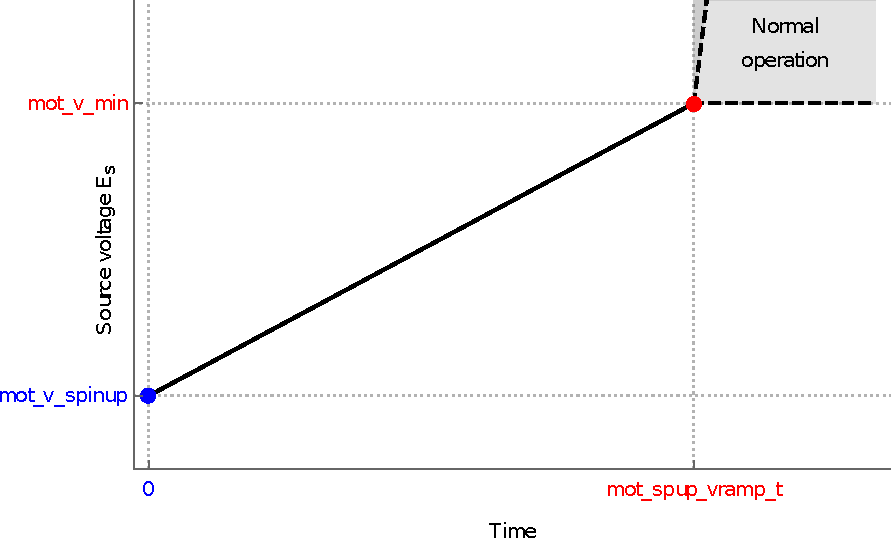
\includegraphics[width=0.7\textwidth]{spinup_voltage_ramp}
	\caption{Voltage ramp during spin-up.
	\label{spinup_voltage_ramp}}
\end{figure}

It should be noted that high initial voltages and/or steep voltage ramps need to be avoided,
because they may lead to severe instabilities in the beginning of the spin-up sequence.
Keep in mind that it is virtually impossible for any synchronous sensorless drive to create stable
torque at low speeds, and especially at standstill.

While spin-up is in progress, Sapog always operates at the zero advance angle
(field weakening disabled) for the reasons explained earlier,
regardless of the configured advance angle settings.

\subsubsection{Spin-up rotor state observer}

The zero crossing detector mentioned above operates in a very different way compared to the
normal rotor state observer used in the normal operating mode.

While operating in spin-up mode, the observable behavior of the induced BEMF may be very erratic,
mainly due to the low magnitude of the signal and irregular rotation of the rotor caused by
imprecise synchronization of the modulated field with the field of the rotor.
In order to combat these difficulties, Sapog employs a different kind of observer, which provides
more robust operation at low speeds.

Immediately after commutation Sapog inserts a blanking delay $T_\text{blank}$
defined by the following equation:
\begin{equation}
T_{\text{blank}}=
\max \left(\frac{\Pi_{\text{blankusec}}}{10^6},
\frac{\Pi_{\text{spupblnkpm}} T_{\text{comm}}}{1000}\right)
\end{equation}
where $\Pi_{\text{spupblnkpm}}$ is the value of the configuration parameter \CfgRef{mot+spup+blnk+pm}
(permill of the commutation period),
$T_{\text{comm}}$ is the duration of the last commutation period,
$\Pi_{\text{blankusec}}$ is the value of the configuration parameter \CfgRef{mot+blank+usec}
(in microseconds).

Upon expiration of the blanking delay, Sapog watches the BEMF waiting for the flyback current to cease.
Afterwards, Sapog starts to integrate the sampled BEMF voltages relative to the neutral voltage.
Once the integrated voltage changes the sign, Sapog switches to the next commutation period.
A more formal definition of the commutation condition is shown below:
\begin{equation}
\begin{aligned}
&\sum_{n} E_{s_n} - E_{\text{neutral}_n} > 0 \qquad\text{for rising BEMF}\\
&\sum_{n} E_{s_n} - E_{\text{neutral}_n} < 0 \qquad\text{for falling BEMF}
\end{aligned}
\end{equation}

The principle is illustrated on the oscillogram \ref{spinup_phase_voltages}.

\begin{figure}[hbt]
    \centering
	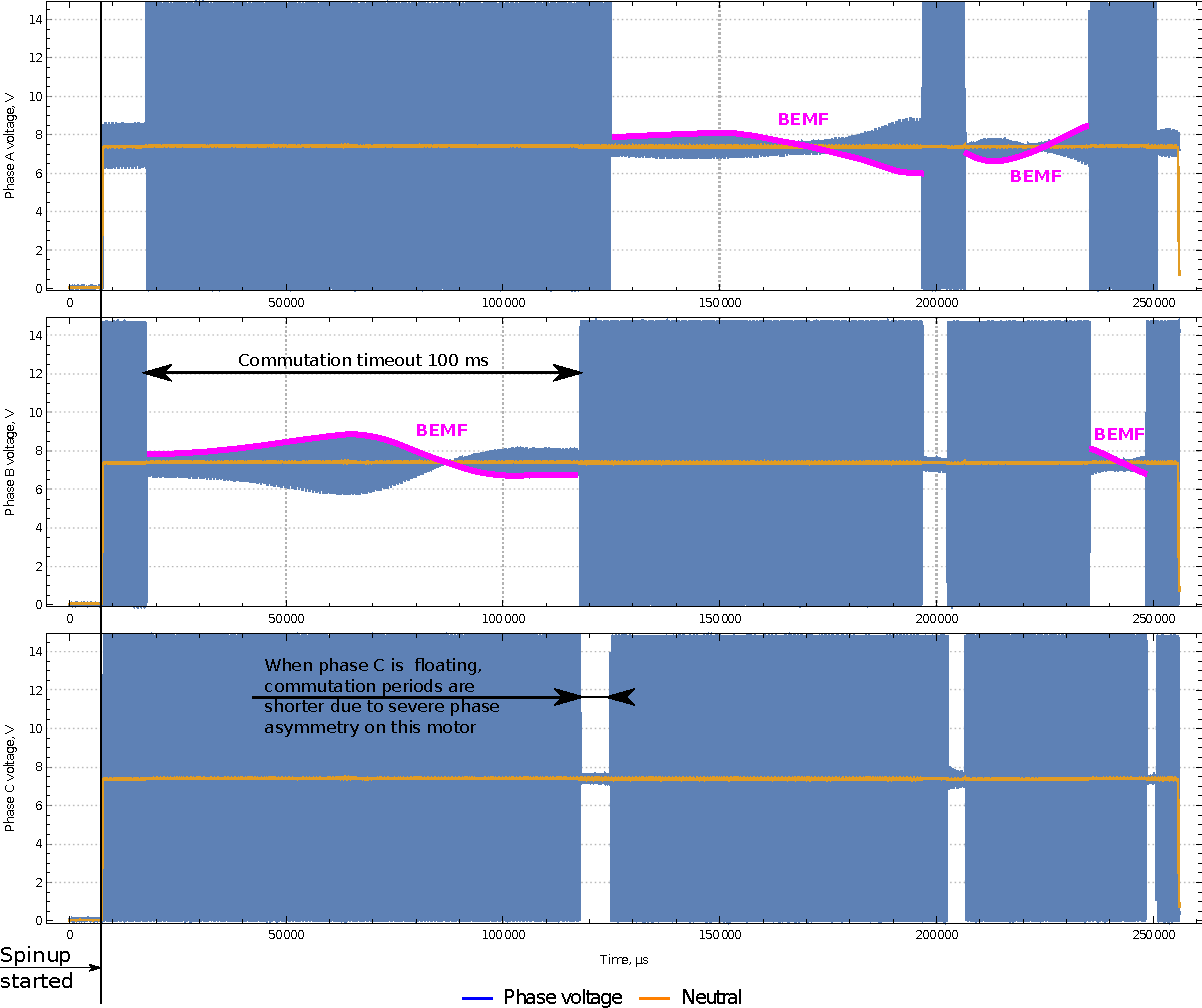
\includegraphics[width=\textwidth]{spinup_phase_voltages}
	\caption{Spin-up sequence with a highly inertial load.
	\label{spinup_phase_voltages}}
\end{figure}

\subsubsection{Termination conditions}

Spin-up will be considered finished once the maximum commutation period defined by the parameter
\CfgRef{mot+comm+per+max} \emph{and} the minimum voltage \CfgRef{mot+v+min} are reached.
Should the target commutation period be reached earlier than the voltage ramp comes to the final
voltage level, the controller will significantly accelerate the ramp in order to converge to
the minimum operating voltage faster.
Once spin-up is finished, the controller will abandon the spin-up mode and switch into normal mode.

If the target commutation period could not be reached in the amount of time specified by
the parameter \CfgRef{mot+spup+to+ms}, in milliseconds, the controller will abort spin-up,
shut down the VSI and register it as a regular rotor stall event.

\subsubsection{Spin-up from non-stationary state}

Sapog assumes that the rotor is (nearly) stationary in the beginning of the spin-up process.
If this assumption is violated, there may be brief transient processes involving abnormal currents,
high vibrations and high EMI.

The transient currents can be either forward or regenerative, depending on whether the desired
and the actual directions of rotation match, and whether the initial guess of the current
commutation step was correct.

Typically Sapog can establish adequate synchronization in a few steps.
If the rotor was rotating in the same direction but at a higher speed,
it will be rapidly decelerated until the speed defined by the load and the source voltage is
reached.
If it is expected that the motor will be frequently started from non-stationary state,
it is recommended to either shorten the initial voltage ramp, or increase the initial
spin-up voltage, in order to reduce the stresses caused by initial braking.

\subsubsection{Configuration parameters}

This section summarizes information about the configuration parameters pertaining to the spin-up mode.
Read the preceding sections for a more detailed review.

\begin{itemize}
\item \CfgRef{mot+spup+blnk+pm} - duration of the extended blanking time during spin-up in permill
(i.e. one-thousands; $10\text{\space{}permill} = 1\% $) of the current commutation period.
\item \CfgRef{mot+spup+to+ms} - overall spin-up timeout, in milliseconds.
If spin-up could not be completed in this amount of time, the rotor will be considered stalled.
\item \CfgRef{mot+spup+st+cp} - maximum commutation period for spin-up mode, in microseconds.
This is also the initial commutation period.
\item \CfgRef{mot+spup+vramp+t} - duration of the initial voltage ramp, in seconds.
\item \CfgRef{mot+v+spinup} - initial source voltage $E_s$ in the beginning of the voltage ramp, in volts.
\end{itemize}

\subsection{Open loop operation}\label{sec:open_loop}

While operating in the open loop mode, Sapog accepts setpoints in the range from 0\% to 100\%,
and treats that as the fraction of the inverter supply voltage $V_\text{inv}$ to
deliver to the motor $E_s$:
\begin{equation}
E_s = V_\text{inv}\cdot{}\mathrm{ramp}\left(\mathrm{limit}\left(S_\text{DC}\right)\right)
\qquad\text{for open loop mode}, S_\text{DC} \in \left(0, 1\right]
\end{equation}
where $S_\text{DC}$ is the setpoint (DC stands for \emph{duty cycle}),
$\mathrm{ramp}$ is the setpoint ramp function,
and $\mathrm{limit}$ is the speed limiting P-controller, reviewed below.

The ramp function replaces abrupt changes in the setpoint with gradual changes.
Abrupt changes that are small enough to not be a hazard to stability of the drive are
accepted by the controller directly, bypassing the ramp.
The following configuration parameters govern the open loop setpoint ramp:

\begin{itemize}
\item \CfgRef{mot+dc+slope} - the slope of the setpoint ramp, in full ranges per second.
For example, the value of 1 allows the controller to sweep the setpoint from 0\% to 100\% in 1 second.
The value of 10 allows the controller to sweep the setpoint from 0\% to 100\% in 0.1 seconds.
\item \CfgRef{mot+dc+accel} - the maximum change in setpoint that will be propagated directly,
bypassing the ramp.
For example, the value of 0.1 allows the controller to apply step changes up to 10\% large directly.
\end{itemize}

Increase the parameters (either one or both) to improve the response characteristics of the drive.
Reduce them if rapid setpoint changes cause stability issues.

Note that the minimum acceptable setpoint is constrained by the minimum duty cycle deduced from
the parameter \CfgRef{mot+v+min}.
If the setpoint falls into $\left(0, S_{\text{DC}_\text{min}}\right]$,
where $S_{\text{DC}_\text{min}}$ is the minimum
duty cycle deduced from the parameter \CfgRef{mot+v+min},
it will be silently overridden to $S_{\text{DC}_\text{min}}$.

The maximum acceptable setpoint will be automatically limited by means of a simple
P-controller\footnote{Proportional controller, i.e. only P term of a PID controller is implemented.}
if the motor approaches the maximum operating speed permitted by the
current PWM carrier frequency, as shown on the figure \ref{pwm_maximum_speed}.

A zero setpoint is treated as the command to stop the motor.
While the motor is stopped, the VSI is disabled, allowing the shaft to rotate freely.

\subsection{RPM control loop}\label{sec:rpm_loop}

When operating in the RPM control mode, also known as RPM governor mode,
Sapog will try to maintain a specified mechanical speed.
Speed control is implemented by means of a parallel PID controller
that takes the current mechanical RPM as input and
produces the duty cycle setpoint at the output.

The nominal update rate of the PID controller $T_{\text{RPMPID}}$ is defined as follows:
\begin{equation}\label{eq:rpm_pid_control_loop_period}
T_{\text{RPMPID}} \approx \max \left(10^{-3},T_{\text{comm}}\right)
\end{equation}
where $T_\text{comm}$ is the current commutation period.
Update of the RPM control loop is not a hard real time process, and the software is allowed to
deviate.

RPM control loop relies on the duty cycle slope control function defined in the section \ref{sec:open_loop},
so the related configuration parameters are still applicable.
The speed limiting P-controller that is used in the open loop mode, however,
is entirely bypassed in RPM mode.
The maximum supported speed is dependent on the PWM carrier frequency;
see the figure \ref{pwm_maximum_speed} for details.
Equation \ref{eq:speed_electrical_mechanical} defines the relation between electrical
and mechanical angular rates.

If the commanded setpoint is lower than the value specified by the parameter \mbox{\CfgRef{mot+rpm+min},}
the actual setpoint will be silently increased to match this value.
A zero setpoint is treated as the command to stop the motor.
While the motor is stopped, the VSI is disabled, allowing the shaft to rotate freely.

The RPM PID controller does not wind up the integral term if the output is constrained by external factors,
such as:
\begin{itemize}
\item Duty cycle ramp.
\item Current limiting controller.
\item Maximum RPM limit.
\end{itemize}

The configuration parameters listed below govern operation of the RPM control loop.
The symbol $\text{DC}$ refers to the duty cycle unit ranging in $\left[-1, 1\right]$,
where negative values correspond to negative inverter source voltage $E_s$.

\begin{itemize}
\item \CfgRef{mot+num+poles} - the number of magnetic poles on the rotor, always even, always $\geq 2$.
This parameter is needed for the controller to convert the electrical speed $\text{RPM}_e$
into mechanical $\text{RPM}_m$.
\item \CfgRef{rpmctl+p} - proportional term of the RPM PID controller,
in $\frac{\text{DC}}{\text{RPM}_m}$.
\item \CfgRef{rpmctl+i} - integral term of the RPM PID controller,
in $\frac{\text{DC}}{\text{second}\cdot{}\text{RPM}_m}$.
\item \CfgRef{rpmctl+d} - derivative term of the RPM PID controller,
in $\frac{\text{second}\cdot{}\text{DC}}{\text{RPM}_m}$.
\item \CfgRef{mot+rpm+min} - minimum mechanical RPM at which stable operation is guaranteed.
\end{itemize}

The overall RPM control loop output for time step $n$ can be approximated with the following equations:
\begin{equation}
e(n) = \omega_{m_{n}} - S_{\omega_{m_{n}}}
\end{equation}
\begin{equation}
E_{s_n} = V_{\text{inv}_n}\cdot\mathrm{ramp}
\left[
\underbrace{\frac{e\left(n\right) - e\left(n-1\right)}{T_{\text{RPMPID}}} \Pi_{\text{rpmctld}}}_\text{derivative} +
\mathrm{clamp}\left(\underbrace{\sum_{i=0}^n e\left(i\right) \Pi_{\text{rpmctli}}}_\text{integral}\right) +
\underbrace{e\left(n\right) \Pi_{\text{rpmctlp}}}_\text{proportional}
\right]
\end{equation}
where:
\begin{itemize}
\item $\mathrm{ramp}$ - slope control function defined in the section \ref{sec:open_loop}.
\item $\mathrm{clamp}$ - integrator wind-up control function described in this section.
\item $\omega_{m}$ - current speed, in mechanical RPM.
\item $S_{\omega_{m}}$ - target speed setpoint, in mechanical RPM.
\item $T_{\text{RPMPID}}$ - instant control loop update period.
See equation \ref{eq:rpm_pid_control_loop_period}.
\item $\Pi_{\text{rpmctlp}}$ - proportional term of the PID controller.
\item $\Pi_{\text{rpmctli}}$ - integral term of the PID controller.
\item $\Pi_{\text{rpmctld}}$ - derivative term of the PID controller.
\end{itemize}

\subsection{Command timeout}\label{sec:setpoint_ttl}

Every setpoint supplied to the motor control logic, regardless of the operating mode, is
accompanied with a time interval that specifies its lifetime - setpoint TTL\footnote{Short for time-to-live.}.
If the time interval expires before the next setpoint is received, Sapog will automatically
stop the motor.

This safety feature ensures that the motor will automatically stop in the event of a communication failure.

The exact duration of the setpoint TTL depends on the communication interface which provides the command.
This is reviewed in detail in the chapter \ref{sec:communication_interfaces}.

\subsection{Current and voltage measurements}

\subsubsection{Measurement}

Sapog measures the DC inverter current $I_\text{inv}$ by means of a current shunt installed on the ground path,
the output of which is connected to the ADC via a current amplifier with a fixed gain coefficient of 10.

The resistance of the current shunt is specified via the configuration parameter \CfgRef{mot+i+shunt+mr},
in milliohms.

The inverter supply voltage $V_\text{inv}$ is measured through a resistor divider with the same
division ratio as that of the BEMF feedback circuits.
This division ratio is hard-coded per every supported hardware design and cannot be changed by the user.

Measurements of the inverter DC current $I_\text{inv}$ and voltage $V_\text{inv}$
are filtered with a first-order low-pass filter.
The corner frequency of the filter is specified by the parameter \CfgRef{mot+lpf+freq}, in hertz.

\subsubsection{Current limiting}\label{sec:current_limiting}

Sapog can limit the maximum DC bus current with the help of a simple P-controller
that activates when the instant current exceeds the limit.
The gain of the current limiting P-controller is specified via the configuration parameter
\CfgRef{mot+i+max+p}, in $\frac{\text{DC}}{\text{ampere}}$, where $\text{DC}$ is the duty cycle units
ranging in $\left[-1, 1\right]$.
The maximum current is specified via the configuration parameter \CfgRef{mot+i+max}, in amperes.

\section{Self diagnostics}\label{sec:self_diagnostics}

Sapog contains a set of diagnostic routines that can detect problems with the hardware.
The diagnostic routines are executed automatically at start up.
Additionally they can be run by external request.

While tests are executed, their progress and status information are printed to the CLI.
The user can understand the nature of detected failures by reading the printed test reports.

If at least one test fails at start-up, the controller will enter panic mode,
where it will remain until power cycled.
Learn more about this in the chapter \ref{sec:indication}.

\subsection{Power stage test}

During the power stage test, Sapog modulates a voltage sequence shown on the table below
and then validates the acquired BEMF samples.
The following legend applies:
\begin{itemize}
\item L - low voltage level. The low side transistor is constantly turned on.
\item H - high voltage level. A high duty cycle PWM is modulated on the phase.
\item F - the phase is floating. Both high and low transistors are turned off.
\end{itemize}

\begin{ZubaxCompactTable}{|c|c c c|}
    Step    & Phase A & Phase B & Phase C \\
    1       & L       & F       & F       \\
    2       & H       & F       & F       \\
    3       & F       & L       & F       \\
    4       & F       & H       & F       \\
    5       & F       & F       & L       \\
    6       & F       & F       & H       \\
\end{ZubaxCompactTable}

The voltage at the output of the BEMF feedback circuits is sampled once for each non-floating phase;
which produces six samples $Q_1 \ldots Q_6$.
Then the following assertions are verified:
\begin{equation}
\begin{aligned}
&Q_1 < L \\
&Q_3 < L \\
&Q_5 < L \\
&Q_2 \approx Q_4 \approx Q_6
\end{aligned}
\end{equation}
where $L$ is a specific lower threshold defined by the hardware implementation,
typically at the level corresponding to 5\% of the dynamic range of BEMF.

The test is considered passed only of all assertions are true.
It is easy to see that this test is invariant to the fact whether the motor is connected or not.

Malfunctions in the following components may cause this test to fail:
\begin{itemize}
\item VSI transistors.
\item VSI transistor drivers.
\item PWM module of the microcontroller.
\item BEMF feedback circuits.
\item ADC module of the microcontroller.
\end{itemize}

\subsection{Phase cross-conductivity test}

The cross-conductivity test allows the controller to detect short-circuits between any of the three
phases or their BEMF feedback circuits.
During this test, the sequence shown in the table below is modulated at the output of the VSI.
The following legend applies:
\begin{itemize}
\item H - high voltage level. A high duty cycle PWM is modulated on the phase.
\item F - the phase is floating. Both high and low transistors are turned off.
\end{itemize}

\begin{ZubaxCompactTable}{|c|c c c|}
    Step    & Phase A & Phase B & Phase C \\
    1       & H       & F       & F       \\
    2       & F       & H       & F       \\
    3       & F       & F       & H       \\
\end{ZubaxCompactTable}

At each step, voltages of all three phases are sampled, which yields the set of samples shown in the next table.
It is assumed that phases that are floating will be pulled down by the resistor dividers in the BEMF feedback
circuits.

\begin{ZubaxCompactTable}{|c|c c c|}
    Step    & Phase A & Phase B & Phase C \\
    1       &$Q_{1A}$ &$Q_{1B}$ &$Q_{1C}$  \\
    2       &$Q_{2A}$ &$Q_{2B}$ &$Q_{2C}$  \\
    3       &$Q_{3A}$ &$Q_{3B}$ &$Q_{3C}$  \\
\end{ZubaxCompactTable}

The following assertions are then validated:
\begin{equation}
\begin{aligned}
&Q_{1A} > H \qquad{} Q_{1B} < L \qquad{} Q_{1C} < L \\
&Q_{2A} < L \qquad{} Q_{2B} > H \qquad{} Q_{2C} < L \\
&Q_{3A} < L \qquad{} Q_{3B} < L \qquad{} Q_{3C} > H \\
\end{aligned}
\end{equation}
where $H$ and $L$ are arbitrary hardware-defined thresholds, high and low, respectively.

Failure of at least one assertion against $H$ indicates that the corresponding phase
or its BEMF feedback circuits are not functioning correctly.
Failure of at least one assertion against $L$ indicates that there is a short circuit between
the current high phase and the phase of the column of the failed assertion.

It is easy to see that the test will always be failing if the motor is connected.
Sapog can recognize that the motor is connected by observing all phases shorted,
in which case the results of this test will be discarded and the test will be considered passed.

\subsection{Inverter voltage and current feedback test}

Over the course of this test, Sapog merely verifies that the measurements reported by the
current and voltage measurement blocks are sane and fall within the expected ranges,
which are hardware-defined.

This test can detect issues with the respective measurement circuits,
ADC, and the power supply of the microcontroller.

\subsection{Temperature monitoring}

Sapog periodically queries the digital temperature sensor installed on the power stage.
This information is reported outside via communication interfaces, but not used
by Sapog itself.

\chapter{Indication}\label{sec:indication}

Sapog is equipped with means of visual and audial indication that are reviewed in this chapter.

\section{RGB LED}

The RGB LED is used to indicate the status of the firmware,
the status of the bootloader while it is running,
or it can be controlled externally via one of the available communication interfaces.
In the latter case, the status indication output is overridden in favor of the externally
received indication commands.

\newcommand{\ShowSolidColor}[1]{%
{\color{#1}\rule{0.4em}{0.8em}\rule{0.4em}{0.8em}\rule{0.4em}{0.8em}\rule{0.4em}{0.8em}\rule{0.4em}{0.8em}}%
}
\newcommand{\ShowBlinkingColor}[1]{{%
\color{#1}\rule{0.4em}{0.8em}%
\color{black}\rule{0.4em}{0.8em}%
\color{#1}\rule{0.4em}{0.8em}%
\color{black}\rule{0.4em}{0.8em}%
\color{#1}\rule{0.4em}{0.8em}%
}}

\subsection{Firmware status indication}

While the firmware is running, the following LED colors can be used to reflect its status.

\begin{ZubaxSimpleTable}{Firmware status indication via RGB LED}{|l l|X|}
    State            &                         & Meaning \\
    Solid white      & \ShowSolidColor{lightgray}& Initialization is in progress, not ready to work yet. \\
    Solid green      & \ShowSolidColor{green}  & Functioning normally. \\
    Blinking cyan    & \ShowBlinkingColor{cyan}& UAVCAN auto-enumeration is in progress, awaiting user input. \\
    Solid yellow     & \ShowSolidColor{yellow} & Controller is locked (see section \ref{sec:stall_detection}),
                                                 or the temperature sensor is malfunctioning. \\
    Solid red        & \ShowSolidColor{red}    & Fatal error, or self test failure.
                                                 Use CLI to obtain detailed info. \\
\end{ZubaxSimpleTable}

\subsection{Bootloader status indication}

The bootloader is started immediately after the device is powered on.
It runs for several seconds, and then, unless there is no valid firmware image
or update of the firmware is requested, the bootloader starts the firmware.
More information on the bootloader and its state indication features
is available in the section \ref{sec:bootloader}.

\subsection{External control}\label{sec:visual_indication_external_control}

The RGB LED can be controlled by external commands via the available communication interfaces.
External control overrides the state indication capabilities of the LED.

\section{Sound}\label{sec:audial_indication}

Sapog can modulate arbitrary sounds by applying specific low-power voltage patterns on the motor windings.
Induced currents cause the windings to vibrate, which produces audible sounds at the frequency of the
applied voltage.

This feature can be invoked by external command via communication interfaces.

At start up, Sapog generates two short beeps with the following parameters:
frequency 1 kHz, duration 100 ms each, spacing 200 ms.

\begin{ZubaxSimpleTable}{Sound modulation capabilities}{|X|c c|l|}
    Parameter                            & Min & Max  & Unit \\
    Audio frequency                      & 100 & 5000 & Hz \\
    Duration of modulated sound          & 1   & 100  & ms \\
\end{ZubaxSimpleTable}

If the requested parameters fall outside the limits specified in the table,
Sapog will automatically constrain the parameters in order to produce the closest achievable results.

Sound modulation requests are only processed if the controller is idle and the motor is stopped.
Otherwise, sound modulation requests will be silently ignored.

\chapter{Communication interfaces}\label{sec:communication_interfaces}

Sapog is equipped with multiple communication interfaces.
Not all communication interfaces can be disabled,
and therefore, more than one interface can be active at the same time.

It is easy to see that this arrangement may lead to issues if more than one
interface is used to command the controller.
Sapog does not attempt to resolve such ambiguity, simply accepting every command
without regard to what interface it was received from.
This trait should be kept in mind when using multiple interfaces concurrently.
For example, a common cause of confusion is encountered when Sapog is connected to a
UAVCAN bus which commands zero setpoint periodically,
and some other interface at the same time is commanding to start the motor.
The controller would appear to behave erratically,
which is caused by alternating conflicting commands.

\section{UAVCAN}

\subsection{Overview}

This section provides documentation for the UAVCAN interface implemented in Sapog.
A general overview and specification of the UAVCAN protocol is provided on the official website at
\url{http://uavcan.org}.

The UAVCAN interface enables access to all features of Sapog.
It is possible to control the motor in all operating modes via UAVCAN,
change the configuration parameters, emit audial and visual indications,
upgrade the firmware, and perform automated ESC enumeration.

This section documents the UAVCAN interface that is available in the firmware itself,
omitting the logic specific to the bootloader, which is documented separately in the chapter
\ref{sec:bootloader}.

Sapog employs Libuavcan - an open source implementation of the UAVCAN protocol stack in C++ distributed under
the MIT software license.

\subsection{Basic functions}

\subsubsection{Node status reporting}

The standard node status message \verb|uavcan.protocol.NodeStatus| is broadcast at 1 hertz.
The mode and health codes are summarized below.

\begin{ZubaxSimpleTable}{UAVCAN node health code interpretation}{|l X|}
Node health & Meaning  \\
OK        & Operating normally. \\
WARNING   & Not used. \\
ERROR     & Not used. \\
CRITICAL  & The controller is locked up (see section \ref{sec:stall_detection}),
            or the temperature sensor is malfunctioning.\\
\end{ZubaxSimpleTable}

\begin{ZubaxSimpleTable}{UAVCAN node mode code interpretation}{|l X|}
Node mode & Meaning  \\
OPERATIONAL        & Operating normally. \\
INITIALIZATION     & The firmware has just started and is not ready to begin normal operation yet. \\
MAINTENANCE        & See the chapter \ref{sec:bootloader} about the bootloader. \\
SOFTWARE\_{}UPDATE & See the chapter \ref{sec:bootloader} about the bootloader. \\
OFFLINE            & Not applicable. \\
\end{ZubaxSimpleTable}

The vendor-specific status code field is not used by Sapog.

Node uptime is reported from the moment when the firmware is started.
The time while the bootloader was running is not included in the reported uptime value.

\subsubsection{Node identification}

The service \verb|uavcan.protocol.GetNodeInfo| is responded to as follows.

All fields of the nested structure \verb|uavcan.protocol.SoftwareVersion|
are populated, which are \verb|major|, \verb|minor|, \verb|vcs_commit|, and \verb|image_crc|.
The VCS commit field is assigned the most significant bits of the git commit hash
of the running revision of the firmware.
The image CRC is computed for the entire firmware image padded to 8 bytes,
with the value of the image CRC value set to zero during CRC computation.

The following fields of the nested structure \verb|uavcan.protocol.HardwareVersion|
are always populated: \verb|major|, \verb|minor|, and \verb|unique_id|.
The values of the fields \verb|major| and \verb|minor| are specific
to the particular hardware model that Sapog is running on.
Please refer to the documentation supplied with your hardware for the specific values.
The field \verb|certificate_of_authenticity| is populated only if any certificate of authenticity
is provided by the vendor.

The field \verb|name| is set to the string \verb|io.px4.sapog|.

\subsubsection{Node restarting}

The service \verb|uavcan.protocol.RestartNode|, if the provided magic number is correct,
unconditionally stops the motor and reboots the controller.
If the provided magic number is incorrect, Sapog returns a response with the field \verb|ok|
set to zero (false).

\subsubsection{Interface statistics}

The service \verb|uavcan.protocol.GetTransportStats| returns the current statistic counters
for both supported CAN interfaces, even if the hardware uses only one of them.
All fields of all nested structures are populated.

\subsubsection{Data type information}

The service \verb|uavcan.protocol.GetDataTypeInfo| provides extensive information about the
supported UAVCAN data types.
No special cases apply.

\subsection{Initialization}

Sapog is a full plug-and-play UAVCAN node that requires no mandatory initial configuration prior to use.

\subsubsection{CAN bus bit rate detection}

Once started, Sapog will automatically detect the bit rate of the CAN bus it is connected to
(if connected to any at all), and remember the detected bit rate until the next boot up.
There is no detection timeout, which means that Sapog can be connected to a CAN bus at
any moment after powering up, and it will configure itself immediately.

It is not possible to specify the bit rate manually.

Sapog requires up to approximately 4 seconds to perform the bit rate detection on a properly
functioning CAN bus.
If the bus is exhibiting erroneous behavior, Sapog may need a longer time to complete the bit rate
detection procedure.

The following bit rates can be detected by Sapog automatically:
\begin{itemize}
\item 1 Mbit/s
\item 500 kbit/s
\item 250 kbit/s
\item 125 kbit/s
\end{itemize}
Sapog cannot be interfaced with a CAN bus that operates at a different bit rate.

Note that if the bootloader (section \ref{sec:bootloader}) was able to detect the bit rate of the CAN bus
before starting the application,
it will pass the detected value over to the application while booting it,
in which case the application will immediately start using the supplied value rather than
performing the bit rate detection again.

\subsubsection{Node ID allocation}

The configuration parameter \CfgRef{uavcan+node+id}, when set to a non-zero value,
defines the node ID of the local UAVCAN node.

If this parameter is set to zero, Sapog will request a dynamic UAVCAN node ID from the bus,
which is the default behavior.

Note that if the bootloader (section \ref{sec:bootloader}) was able to obtain a dynamic UAVCAN node ID
from the bus before starting the application,
it will pass the detected value over to the application while booting it,
in which case the application will use the provided node ID
\emph{regardless of the value configured in \CfgRef{uavcan+node+id}}.

Until there is a valid node ID available for the local UAVCAN node (either specified
statically via the configuration parameter, or provided dynamically),
no other functions of the UAVCAN interface will work.
This implies, for example, that it is not possible to control the motor via UAVCAN
until the local node is fully configured.

\subsection{Motor control}

\subsubsection{Setpoint input}

Motor control is governed by means of two standard message types that Sapog subscribes to.
The message \verb|uavcan.equipment.esc.RawCommand| puts Sapog into the open loop control mode
(section \ref{sec:open_loop}).
The message \verb|uavcan.equipment.esc.RPMCommand| puts Sapog into the RPM loop control mode
(section \ref{sec:rpm_loop}).

Both messages carry arrays of commands for multiple motors.
Sapog selects the single command from the array at the index specified by the configuration
parameter \CfgRef{esc+index}.
If the specified index points out of the range of the array,
Sapog assumes that the commanded setpoint is zero, and stops the motor.\footnote{
Obviously, multiple ESC can share the same ESC index setting.}

Sapog does not perform any additional processing of the received command message,
and does not prioritize between the supported types of messages
and between different broadcasters.
This means that the drive will not operate properly if there are multiple types of control
messages being received, or if multiple nodes are broadcasting conflicting setpoints.
Direct execution of received commands without additional processing allows Sapog to achieve
minimal response latency and high command throughput.

Setpoints received via UAVCAN are assigned a fixed lifetime, which is specified by the
configuration parameter \CfgRef{cmd+ttl+ms}.
Read more on the concept of setpoint TTL in the section \ref{sec:setpoint_ttl}.

As a safety precaution, when the motor is stopped and a non-zero open loop setpoint is received,
Sapog will refuse to start the motor if the received non-zero open loop setpoint exceeds the
threshold value specified by the configuration parameter \CfgRef{cmd+start+dc},
in the duty cycle units.
This feature helps the user to avoid starting the motor accidentally to a high power level,
for example, due to a failure in the system that controls Sapog.
This feature is only available for the open loop control mode.

\subsubsection{Status reporting}

The standard message type \verb|uavcan.equipment.esc.Status| is used to report status of the
motor control system.
The message is broadcast at 1 hertz if the motor is not running,
and at 10 hertz if the motor is starting or running.
All fields of the message are populated.

The field \verb|error_count| carries the number of failures to detect a valid zero crossing
point since the motor has started.
The error counter may overflow if the motor is running without stopping for a very long time,
although this will never happen as long as the drive is functioning correctly.

The field \verb|esc_index| contains the value of the configuration parameter \CfgRef{esc+index}.

\subsection{Configuration parameter management}

The standard UAVCAN configuration parameter management interface is supported
by means of the service data types defined in the namespace \verb|uavcan.protocol.param|.

Note that the save action available via the service \verb|uavcan.protocol.param.ExecuteOpcode|
is supported, but is redundant, because Sapog commits all the configuration parameters
to the non-volatile configuration storage memory automatically after modification.

When obtaining the list of all available configuration parameters using the field \verb|index|
of the service \verb|uavcan.protocol.param.GetSet|, the ordering of the returned configuration
parameters is undefined, but it is guaranteed to be consistent within the same firmware build.
Updating the firmware to different versions or even different builds of the same version
may change the ordering of the configuration parameters.

\subsection{Audial and visual indication}

\subsubsection{Audial indication}

The standard message type \verb|uavcan.equipment.indication.BeepCommand|
can be used to invoke the audial indication feature of Sapog
described in the section \ref{sec:audial_indication}.

\subsubsection{RGB LED control}

The standard message type \verb|uavcan.equipment.indication.LightsCommand|
can be used to control the RGB LED indicator via UAVCAN, as described in the section 
\ref{sec:visual_indication_external_control}.

The configuration parameter \CfgRef{light+index} defines the UAVCAN light ID of the RGB LED.
Light control commands will only be accepted if the value of the field \verb|light_id|
matches the value stored in the configuration parameter \CfgRef{light+index}.

\subsection{Firmware upgrade}

The service \verb|uavcan.protocol.file.BeginFirmwareUpdate| reboots the device into the bootloader
mode.
The bootloader mode is documented in the chapter \ref{sec:bootloader}.

If the motor is running at the time of reception of this request, it is stopped unconditionally.

Note that the request argument \verb|image_file_remote_path| is always ignored.
It is therefore required to invoke this service again after the firmware has entered the bootloader
(i.e. about $3\pm{}1$ seconds after the first invocation),
otherwise the upgrade process will not begin.
This requirement may be removed in the future.

\subsection{Automated ESC enumeration}

Sapog allows the user to configure the ESC index (parameter \CfgRef{esc+index})
and the direction of rotation (parameter \CfgRef{ctl+dir}) intuitively,
by means of manual rotation of the rotors in a specific order and direction.
This feature is only useful for multi-motor vehicles, such as multirotor UAV,
and is entirely optional.
The respective configuration parameters can be equally well configured manually
by the user, instead of resorting to this more sophisticated method.

The UAVCAN namespace \verb|uavcan.protocol.enumeration| contains the data type definitions that
this feature is based upon.

When invoking the automated enumeration sequence, the field \verb|parameter_name|
of the service type \verb|uavcan.protocol.enumeration.Begin| should be left empty
(which means ``parameter name auto-detect'' according to the UAVCAN specification).

The user indication input is provided by means of turning the rotor manually in the normal
direction of rotation.
Sapog will memorize the direction of rotation and reflect it in the corresponding configuration
parameter.

Enumeration request will return the error \verb|ERROR_INVALID_MODE| if the motor is not stopped.

The user can benefit from this feature only if there is an adequate support from the
controlling hardware installed on the vehicle (e.g. autopilot).
Therefore, the full description of this feature falls outside of the scope of this
manual.
For reference, the process of automated ESC enumeration performed with the PX4 autopilot
is demonstrated on the following video: \url{https://youtu.be/4nSa8tvpbgQ}.

\subsection{Data type summary}

\begin{ZubaxSimpleTable}{UAVCAN broadcast messages}{|l l l X|}
    Data type name                                         & Frequency, Hz & Tr. priority & Note \\
    \texttt{uavcan.protocol.NodeStatus}                    & 1          & 16 (medium)  & \\
    \texttt{uavcan.protocol.dynamic\_node\_id.Allocation}  & Aperiodic  & 30 (low)     & Only during the
                                                                                         initialization or while
                                                                                         in the bootloader. \\
    \texttt{uavcan.protocol.enumeration.Indication}        & Aperiodic & 16 (medium)   & Only during ESC
                                                                                         enumeration. \\
    \texttt{uavcan.equipment.esc.Status}                   & 1 or 10   & 16 (medium)   & 1 Hz while idle,
                                                                                         10 Hz otherwise. \\
    \texttt{uavcan.protocol.debug.LogMessage}              & Aperiodic & 31 (lowest)   & \\
\end{ZubaxSimpleTable}

\begin{ZubaxSimpleTable}{UAVCAN subscribed messages}{|l X|}
    Data type name                                         & Note \\
    \texttt{uavcan.protocol.dynamic\_node\_id.Allocation}  & Only during the initialization or while
                                                             in the bootloader. \\
    \texttt{uavcan.equipment.esc.RawCommand}               & Open loop setpoint. \\
    \texttt{uavcan.equipment.esc.RPMCommand}               & RPM control loop setpoint. \\
    \texttt{uavcan.equipment.indication.BeepCommand}       & Ignored if the motor is running. \\
    \texttt{uavcan.equipment.indication.LightsCommand}     & Overrides the RGB LED state indication. \\
\end{ZubaxSimpleTable}

\begin{ZubaxSimpleTable}{UAVCAN provided services}{|l X|}
    Data type name                                         & Note \\
    \texttt{uavcan.protocol.GetNodeInfo}                   & \\
    \texttt{uavcan.protocol.GetDataTypeInfo}               & \\
    \texttt{uavcan.protocol.GetTransportStats}             & \\
    \texttt{uavcan.protocol.RestartNode}                   & \\
    \texttt{uavcan.protocol.enumeration.Begin}             & Returns error if the motor is running. \\
    \texttt{uavcan.protocol.file.BeginFirmwareUpdate}      & Stops the motor and reboots into the bootloader. \\
    \texttt{uavcan.protocol.param.ExecuteOpcode}           & \\
    \texttt{uavcan.protocol.param.GetSet}                  & \\
\end{ZubaxSimpleTable}

\section{CLI}

\subsection{Overview}

Sapog provides a plain text command line interface (CLI) over its serial port interface.
The CLI can be used for user interaction directly, or it can be used as a machine-to-machine command interface,
since the command and response syntax is quite simple.

The serial port interface operates at 115200 baud, 8 bit per word, no parity control, one stop bit
(115200-8N1).

The CLI line ending is \verb|\r\n| (CR, LF).

Barring any special preferences,
it is recommended to use the software listed in the table \ref{cli_software_recommendations}
for accessing the CLI from the user's PC.

\begin{ZubaxSimpleTable}{CLI terminal emulators}{|l l X|}\label{cli_software_recommendations}
    PC OS            & Application         & Note \\
    GNU/Linux        & \texttt{picocom}    & A simple and robust command-line tool.
                                             It should be preferred over the popular
                                             \texttt{minicom} and \texttt{screen}. \\
    MS Windows       & PuTTY               & A simple multi-purpose GUI terminal emulator.
                                             The HyperTerminal tool supplied by default with some versions
                                             of Windows should be avoided. \\
\end{ZubaxSimpleTable}

\subsection{Boot logging}

While in the process of booting, Sapog prints human-readable diagnostic messages via the serial port interface.
The printed messages, among other things, include the reports of the start-up self-test procedures
described in the section \ref{sec:self_diagnostics}.

Normally the boot-up messages should only be of interest for troubleshooting purposes.

\subsection{Panic reporting}

If Sapog encounters a catastrophic failure that renders it dysfunctional
(e.g. a memory access violation, stack overflow, failure of the computing hardware, etc),
it uses the serial interface as a last resort status reporting option.
In this case, Sapog will dump as much status information as possible into the serial port,
after which it will lock up and wait for the watchdog timer to reset it.

\subsection{CLI commands}

This section documents the CLI commands that can be of interest to the end user.
Some commands that are not intended for use in production are intentionally omitted from this reference.

\subsubsection{help}

Prints the list of all available commands.

\subsubsection{cfg}

This command provides access to the configuration parameter storage.
The configuration parameters and their non-volatile storage are described in more detail in the chapter
\ref{sec:configuration_parameters}.

Syntax:
\begin{itemize}
    \item \verb|cfg list| - list all configuration parameters, their current values,
          acceptable value intervals, and default values.
    
    \item \verb|cfg save| - save the current configuration into the non-volatile storage.
          This command is redundant and normally need not be used, because Sapog commits all configuration
          into the non-volatile storage automatically upon modification.
    
    \item \verb|cfg erase| - erase the current configuration and reset the non-volatile memory to factory defaults.
    
    \item \verb|cfg set <name> <value>| - assign the configuration parameter named \verb|<name>| the value
          \verb|<value>|. For example: \verb|cfg set foo 42|.
          The non-volatile storage will be updated automatically.
\end{itemize}

The syntax \verb|cfg list| prints one parameter per line, where the line is formatted as follows:

\verb|name = value [min, max] (default)|

The number of whitespaces between tokens may vary.

Floating point parameters are always reported with the point symbol (\verb|.|),
which allows one to distinguish them from integer and boolean typed parameters.

Boolean parameters are reported as integers, where 1 represents logical true and 0 represents logical false.
They can be distinguished from integer parameters by their minimum and maximum values being 0 and 1,
respectively.

Whenever a parameter is assigned a new value, the device verifies if the new value is within the
acceptable limits.
If it is, the new value is assigned. Otherwise, the old value is retained.
Afterwards the device prints out the resulting value of the parameter in the following format:

\verb|name = value|

The number of whitespaces between tokens may vary.

This response can be used to check whether the new value has been accepted by the device or not.

\subsubsection{reboot}

Reboot the firmware.
If the motor is running, it will be stopped first.

\subsubsection{beep}

Modulate sound as described in the section \ref{sec:audial_indication}.

Syntax:
\begin{itemize}
\item \verb|beep| - emit sound of the default duration at the default frequency.
\item \verb|beep <freq>| - modulate sound of the default duration at the frequency \verb|<freq>|
specified in hertz. For example: \verb|beep 1000|.
\item \verb|beep <freq> <dur>| - modulate sound of the specified duration \verb|<dur>| in milliseconds
at the frequency \verb|<freq>| specified in hertz. For example: \verb|beep 5000 200|.
\end{itemize}

\subsubsection{stat}

Print the current state of the motor controller in a human-readable form.
At least the following information will be displayed:
\begin{itemize}
\item Inverter supply voltage.
\item Inverter DC current.
\item Mechanical RPM.
\item Actual duty cycle (not the setpoint).
\item The number of failures since the motor has started.
\end{itemize}

\subsubsection{test}

Execute the self-test routines, described in the section \ref{sec:self_diagnostics}.
The output will be printed in a human-readable format.

\subsubsection{dc}

Set the open loop control setpoint.
See the section \ref{sec:open_loop} for more information about the open loop control mode.

The setpoint TTL when using this command is fixed at 30 seconds.
More information on the setpoint TTL feature is provided in the section \ref{sec:setpoint_ttl}.

By default this command is locked for safety reasons.
In order to unlock it, execute \verb|dc arm| once, and it will stay unlocked until the firmware is rebooted.

Syntax:
\begin{itemize}
\item \verb|dc| - assign zero setpoint, which will stop the motor if it is running.
\item \verb|dc arm| - unlock the command.
\item \verb|dc <duty cycle>| - set the specified duty cycle setpoint.
The setpoint is a real number in the interval $\left[0, 1\right]$.
For example: \verb|dc 0.5| assigns the 50\% duty cycle.
\end{itemize}

\subsubsection{rpm}

Set the RPM control loop setpoint.
See the section \ref{sec:rpm_loop} for more information about the RPM control mode.

The setpoint TTL when using this command is fixed at 30 seconds.
More information on the setpoint TTL feature is provided in the section \ref{sec:setpoint_ttl}.

By default this command is locked for safety reasons.
In order to unlock it, execute \verb|rpm arm| once, and it will stay unlocked until the firmware is rebooted.

Syntax:
\begin{itemize}
\item \verb|rpm| - assign zero setpoint, which will stop the motor if it is running.
\item \verb|rpm arm| - unlock the command.
\item \verb|rpm <RPM>| - set the specified RPM setpoint.
The setpoint is an integer number in the interval $\left[0, 65535\right]$.
For example: \verb|rpm 5000| assigns the target setpoint of 5000 mechanical RPM.
\end{itemize}

\subsubsection{md}

Print the internal motor controller status information in a human-readable format.
The output of this command is also printed automatically when the rotor gets stalled.

\subsubsection{zubax\_id}\label{sec:cli_zubax_id}

This command reports the complete information identifying this particular product:
type, version information, make and model.
The information is printed in a machine-readable yet human-friendly
YAML\footnote{\url{https://en.wikipedia.org/wiki/YAML}} format.

An example output is shown in the following listing.
The meaning of each well-defined field is explained in the table \ref{zubax_id_fields_table}.
Fields that are not intended for production use are intentionally left undocumented.
Note that the number of fields and their ordering may vary.

\begin{minted}{yaml}
product_id   : 'io.px4.sapog'
product_name : 'PX4 Sapog'
sw_version   : '2.0'
sw_vcs_commit: 7672820
sw_build_date: Apr 29 2017
hw_version   : '1.1'
hw_unique_id : 'M//UBUdHNTZUVxlDAAAAAA=='
hw_signature : 'NX3Y05Y1a/hDNajPyMF5dojuAB9r1HmUxZ3UVU8g39C9L5pjAZMVKdZ7yI1CetvumOJZHIjRYkHOBmMAEKvRU/3mpG\
+KgUND6yGpoHQ5aa+OK+LIcOw2LC+BaUmAPS6Hy4bxOvuARb062QruQlrOXyVc/vs28JtcBzOZo/b/OxY='
hw_info_url  : 'http://device.zubax.com/device_info?uid=33FFD405474735365457194300000000'
\end{minted}

\begin{ZubaxSimpleTable}{Zubax ID fields}{|l X|}\label{zubax_id_fields_table}
Field name              & Meaning \\

\texttt{product\_id}    & Product type identifier string. It is always set to \texttt{io.px4.sapog}.
The same string is reported via UAVCAN as the node name string. \\

\texttt{sw\_version}    & Firmware version number in the form ``major.minor''. \\

\texttt{sw\_vcs\_commit}& Firmware patch ID as the short git commit hash.
The abbreviation VCS stands for ``version control system''.
This number allows to pinpoint the exact revision of the firmware that is currently running. \\

\texttt{sw\_build\_date}& Firmware build date in the form ``\texttt{mmm dd yyyy}''. \\

\texttt{hw\_version}    & Hardware version number in the form ``major.minor''.
Refer to the documentation provided with your hardware to learn what version number it reports to Sapog. \\

\texttt{hw\_unique\_id} & The 128-bit unique ID of this specific hardware instance.
The UID is represented either as a hexadecimal string, or as a Base64 encoded string.\\

\texttt{hw\_signature}  & The certificate of authenticity (CoA) of this specific hardware instance
encoded in a Base64 string.
This field will not be present if the current hardware instance does not have any CoA installed.
Refer to the documentation provided with your hardware to find out what CoA is used, if any. \\

\texttt{hw\_info\_url}  & Link to the web page that contains the test report, origin information,
traceability data, and other important information about this specific hardware instance provided by
the vendor. This field may not be populated if the hardware does not have any CoA installed. \\

\end{ZubaxSimpleTable}

Vendors that use Sapog for their own products can use this command to install their own CoA onto the hardware.
Beware that the CoA can be written only once.
The following form is used to write the CoA: \verb|zubax_id <CoA>|,
where \verb|<CoA>| is a placeholder for Base64 encoded certificate of authenticity.
More information about using Sapog in custom products is provided in the chapter \ref{sec:porting_guide}.

Syntax:
\begin{itemize}
\item \verb|zubax_id| - print the Zubax ID YAML structure documented above.
\item \verb|zubax_id <CoA>| - install the vendor's certificate of authenticity \verb|<CoA>| encoded in Base64.
This command can be executed only once.
\end{itemize}

\subsubsection{uavcan}

Print the status information of the local UAVCAN stack in a human-readable format.
This command may take several seconds to execute, depending on the state of the UAVCAN stack.

\section{RCPWM}

\subsection{Overview}

RCPWM is a simple analog interface that encodes the command in a series of repeating pulses.
The commanded setpoint is proportional to the duration of the pulses,
whereas the spacing between the pulses and their interval do not carry any useful information.
The principle is illustrated on the figure \ref{rcpwm_signal_plot}.

\begin{figure}[hbt]
    \centering
	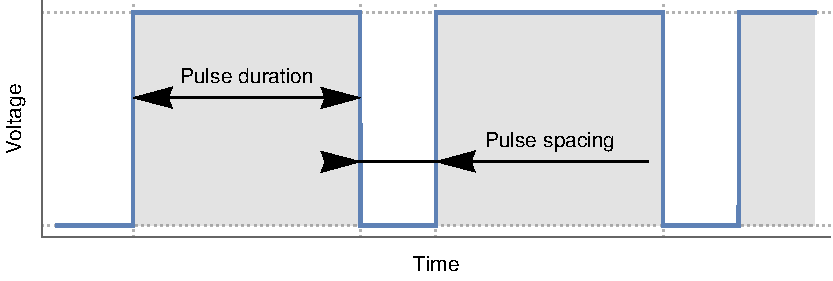
\includegraphics[width=0.7\textwidth]{rcpwm_signal_plot}
	\caption{RCPWM signal.
	\label{rcpwm_signal_plot}}
\end{figure}

The RCPWM interface is widely used in robotics and flight control systems of small UAV.
Its obvious downsides are the lack of any kind of feedback from the controlled system,
very low throughput,
high latency (in excess of 2 milliseconds in certain scenarios, and never lower than 1 millisecond),
and general physical inefficiency due to the need to use one independent electrical connection
per controlled system.

\subsection{Functional description}

When the RCPWM interface is enabled, Sapog demodulates the RCPWM signal into the open loop mode setpoints,
and feeds them into the motor controller.
Setpoints received via RCPWM are accepted immediately without pre-filtering or any other preprocessing.

In order to be understood by Sapog,
the RCPWM signal should match the requirements listed in the table \ref{rcpwm_constraints}.

\begin{ZubaxSimpleTable}{RCPWM interface constraints}{|c X|c c|c|}\label{rcpwm_constraints}
Symbol                               & Parameter            & Min   & Max & Unit \\
$\Delta{}t_{\text{HL}_\text{RCPWM}}$ & RCPWM pulse duration & 0.5   & 3   & millisecond \\
$\Delta{}t_{\text{LH}_\text{RCPWM}}$ & RCPWM pulse spacing  & 0.01  & 50  & millisecond \\
\end{ZubaxSimpleTable}

If the RCPWM pulse duration $\Delta{}t_{\text{HL}_\text{RCPWM}}$ is not within the specified limits,
Sapog treats it as if there was no modulation at all.

The setpoint TTL for RCPWM commands is fixed at 100 milliseconds.
This implies that the motor will be stopped in 100 milliseconds after the RCPWM modulation is gone.
More information on the setpoint TTL feature is provided in the section \ref{sec:setpoint_ttl}.

The configuration parameter \CfgRef{pwm+enable} specifies whether the RCPWM is active.
If the interface is disabled, Sapog will ignore the state of the RCPWM input line.
If the interface is enabled, care should be taken to ensure that no conflicting commands
are being issued via the other interfaces, otherwise the controller may exhibit an erratic behavior.

The configuration parameters \CfgRef{pwm+min+usec} and \CfgRef{pwm+max+usec} define the pulse duration
that corresponds to the minimum (zero) and the maximum (100\%) setpoints, respectively, in microseconds.
Pulses shorter than \CfgRef{pwm+min+usec} are translated to zero setpoint;
likewise, pulses that are longer than \CfgRef{pwm+max+usec} are translated to the maximum setpoint.

Sapog applies a start-stop hysteresis that works as follows: if the motor is stopped, it will not start
until the commanded setpoint has exceeded 6\%.
If the motor is running, it will not stop until the commanded setpoint has fell below 3\%.

A safety feature will not allow the motor to start if the commanded setpoint exceeds 40\%.
Therefore, combining the effects of the hysteresis feature and the safety threshold,
it can be seen that the motor will start only if the commanded setpoint falls into the interval
$\left(6\%, 40\%\right)$.

The setpoint handling logic is illustrated on the figure \ref{rcpwm_setpoint_handling}.

\begin{figure}[hbt]
    \centering
	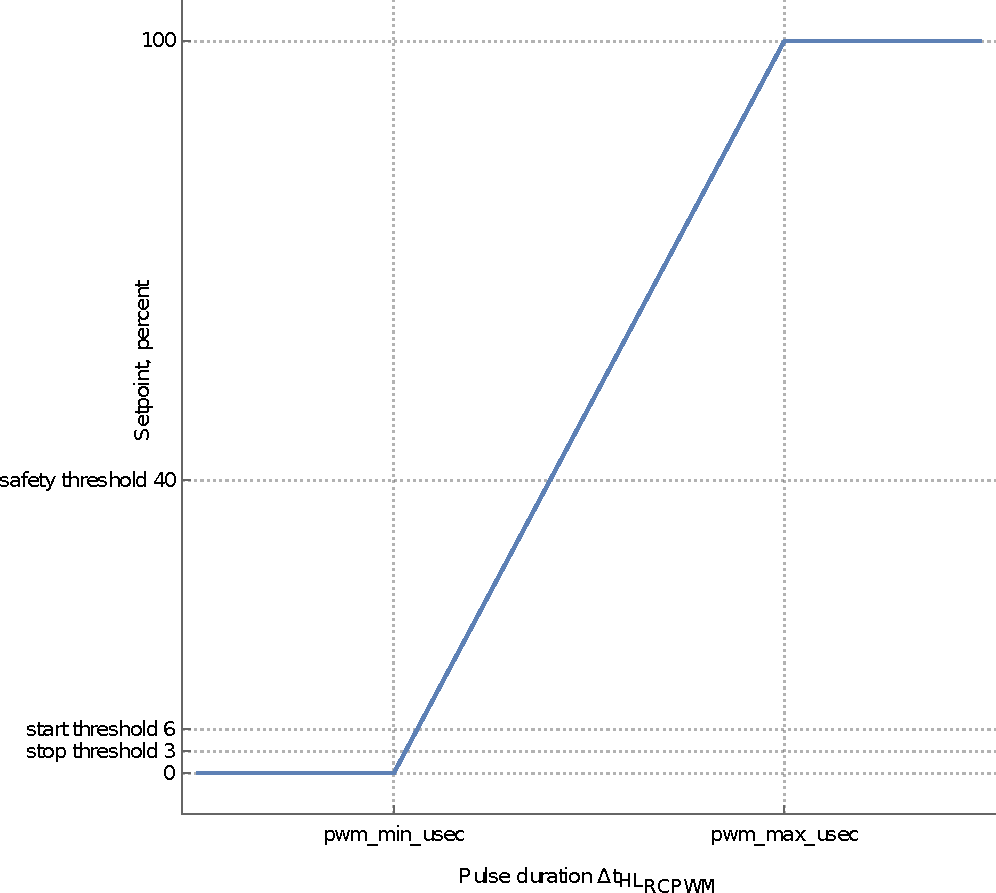
\includegraphics[width=0.8\textwidth]{rcpwm_setpoint_handling}
	\caption{RCPWM setpoint handling.
	\label{rcpwm_setpoint_handling}}
\end{figure}

\chapter{Configuration parameters}\label{sec:configuration_parameters}

This chapter summarizes all configuration parameters available in Sapog.

The length of the configuration parameter names does not exceed 16 characters,
which ensures compatibility with MAVLink version 1.

\section{Non-volatile configuration storage}

All configuration parameters are stored in a non-volatile memory
that retains its contents across power cycles.

Modification of any single parameter will trigger Sapog to commit all of them into the non-volatile
memory one second after the last modification has taken place.
The one second delay ensures that no excessive modifications of the non-volatile memory will be carried out
when multiple configuration parameters are changed at the same time.

Sapog will not write or erase the non-volatile memory as long as the motor is running, in order to
avoid interference with the hard real time motor control algorithms.
If configuration was changed while the motor is running,
a write operation will be postponed until the motor is stopped.

If the device is turned off while the configuration storage was being updated,
the stored configuration data may get damaged.

The stored configuration is read from the non-volatile memory once upon boot-up.
If Sapog detects that the stored configuration data has been damaged,
it will automatically revert to the factory default configuration.
Sapog can always reliably detect damage of the stored configuration data,
so it is guaranteed that invalid configuration can never be loaded.

\section{Firmware upgrade considerations}

Configuration parameters of different revisions of the firmware may be incompatible with each other.
For instance, some configuration parameters may be added, removed, or their value intervals may be changed.

Sapog always checks whether the stored configuration data is compatible with the current firmware revision.
If it is detected that the stored configuration cannot be applied to the current version of the firmware,
Sapog will automatically revert to the factory default configuration.

Keep these considerations in mind when upgrading the firmware.

\section{Configuration parameter index}

The minimum, maximum, and default values provided in the table are shown for exemplary purposes only,
and they are \emph{not expected to be valid} for all firmware revisions that this document applies to.
Intervals and default values may change in newer firmware revisions; furthermore,
they can also depend on which particular hardware Sapog is running on.

The following abbreviations are adopted for the tables below:
\begin{description}
\item[TEA] Short for ``takes effect at''. This field specifies when the newly specified parameter value will
take effect.
\item[Def.] Short for ``default value''.
\end{description}

% name, unit, takes effect at, min, max, default, note
\newcommand\CfgParamIndexEntry[7]{%
    \CfgDef{#1} & \footnotesize{#2} & \footnotesize{\CfgListReferences{#1}} & \footnotesize{#3} &
    \footnotesize{#4} & \footnotesize{#5} & \footnotesize{#6} &
    \footnotesize{#7} \tabularnewline
}%

\newenvironment{CfgParamIndex}[1]{%
    \begin{ZubaxTableWrapper}{#1}
    \setlength\tabcolsep{2.5pt}
    \begin{ZubaxWrappedTable}{@{} l l l l | c c c | X @{}}
    Name & Unit & Pages & TEA & Min & Max & Def. & Description \\
}{%
    \end{ZubaxWrappedTable}
    \end{ZubaxTableWrapper}
}

\subsection{Motor control configuration parameters}

\begin{CfgParamIndex}{Motor control configuration parameters}
\CfgParamIndexEntry{mot+pwm+dt+ns}{nanosecond}{boot}{400}{800}{}{PWM dead time}
\CfgParamIndexEntry{mot+pwm+hz}{hertz}{boot}{20000}{75000}{60000}{PWM carrier frequency}
\CfgParamIndexEntry{mot+spup+blnk+pm}{permill}{boot}{1}{300}{100}{Min blanking time during spin-up}
\CfgParamIndexEntry{mot+spup+to+ms}{millisecond}{boot}{100}{9000}{5000}{Spin-up timeout}
\CfgParamIndexEntry{mot+spup+st+cp}{microsecond}{boot}{10000}{300000}{100000}{Spin-up max/initial comm. period}
\CfgParamIndexEntry{mot+comm+per+max}{microsecond}{boot}{1000}{10000}{4000}{Max comm. period for normal mode}
\CfgParamIndexEntry{mot+zc+fails+max}{}{boot}{6}{300}{20}{Stall detection threshold}
\CfgParamIndexEntry{mot+bemf+range}{percent}{boot}{10}{100}{90}{Valid BEMF magnitude}
\CfgParamIndexEntry{mot+bemf+win+den}{}{boot}{3}{8}{4}{BEMF sampling window length denominator}
\CfgParamIndexEntry{mot+blank+usec}{microsecond}{boot}{10}{300}{40}{Comm. blanking time for normal mode}
\CfgParamIndexEntry{mot+tim+cp+min}{microsecond}{boot}{100}{50000}{600}{Advance angle interpolation point}
\CfgParamIndexEntry{mot+tim+cp+max}{microsecond}{boot}{100}{50000}{300}{Advance angle interpolation point}
\CfgParamIndexEntry{mot+tim+adv+max}{angular degree}{boot}{0}{29}{15}{Advance angle interpolation point}
\CfgParamIndexEntry{mot+tim+adv+min}{angular degree}{boot}{0}{20}{5}{Advance angle interpolation point}
\CfgParamIndexEntry{mot+i+shunt+mr}{milliohm}{boot}{0.1}{100}{}{Resistance of the current measurement shunt}
\CfgParamIndexEntry{rpmctl+p}{$\frac{\text{dutycycle}}{\text{RPM}_m}$}{boot}{0}{1}{0.0001}%
{RPM loop PID proportional gain}
\CfgParamIndexEntry{rpmctl+i}{$\frac{\text{dutycycle}}{\text{second}\cdot\text{RPM}_m}$}{boot}{0}{10}{0.001}%
{RPM loop PID integral gain}
\CfgParamIndexEntry{rpmctl+d}{$\frac{\text{second}\cdot\text{dutycycle}}{\text{RPM}_m}$}{boot}{0}{1}{0}%
{RPM loop PID derivative gain}
\CfgParamIndexEntry{mot+stop+thres}{}{boot}{1}{100}{7}{Lock-up threshold}
\CfgParamIndexEntry{mot+lpf+freq}{hertz}{boot}{1}{200}{20}{Current/voltage low-pass filter corner frequency}
\CfgParamIndexEntry{mot+i+max}{ampere}{boot}{1}{60}{20}{Maximum inverter current}
\CfgParamIndexEntry{mot+i+max+p}{$\frac{\text{dutycycle}}{\text{ampere}}$}{boot}{0.01}{2}{0.2}%
{Current limiter proportional gain}
\CfgParamIndexEntry{mot+rpm+min}{RPM}{boot}{50}{5000}{1000}{Minimum setpoint for RPM control loop}
\CfgParamIndexEntry{ctl+dir}{}{boot}{0}{1}{0}{Direction of rotation: 0 - forward, 1 - reverse}
\CfgParamIndexEntry{mot+num+poles}{}{boot}{2}{100}{14}{Number of magnetic poles on the rotor}
\CfgParamIndexEntry{mot+dc+slope}{$\frac{\text{dutycycle}}{\text{second}}$}{boot}{0.1}{20}{5}%
{Duty cycle ramp steepness}
\CfgParamIndexEntry{mot+dc+accel}{duty cycle}{boot}{0.001}{0.5}{0.09}{Duty cycle ramp bypass threshold}
\CfgParamIndexEntry{mot+spup+vramp+t}{second}{boot}{0}{10}{3}{Duration of spin-up voltage ramp}
\CfgParamIndexEntry{mot+v+spinup}{volt}{boot}{0.01}{10}{0.5}{Initial voltage of spin-up voltage ramp}
\CfgParamIndexEntry{mot+v+min}{volt}{boot}{0.5}{10}{2.5}{Min inverter source voltage for normal mode}
\end{CfgParamIndex}

\subsection{UAVCAN interface configuration parameters}

\begin{CfgParamIndex}{UAVCAN interface configuration parameters}
\CfgParamIndexEntry{esc+index}{}{boot}{0}{15}{0}{UAVCAN index of this ESC}
\CfgParamIndexEntry{cmd+ttl+ms}{millisecond}{boot}{100}{5000}{200}{Setpoint timeout}
\CfgParamIndexEntry{cmd+start+dc}{duty cycle}{boot}{0.01}{1}{1}{Spin-up safety threshold}
\CfgParamIndexEntry{uavcan+node+id}{}{boot}{0}{125}{0}{Node ID, zero for dynamic allocation}
\CfgParamIndexEntry{light+index}{}{boot}{0}{255}{0}{UAVCAN index of the RGB LED}
\end{CfgParamIndex}

\subsection{RCPWM interface configuration parameters}

\begin{CfgParamIndex}{RCPWM interface configuration parameters}
\CfgParamIndexEntry{pwm+max+usec}{microsecond}{boot}{1800}{2200}{2000}{Full throttle pulse duration}
\CfgParamIndexEntry{pwm+min+usec}{microsecond}{boot}{800}{1200}{1000}{Zero throttle pulse duration}
\CfgParamIndexEntry{pwm+enable}{}{boot}{0}{1}{0}{Enable this interface}
\end{CfgParamIndex}

\subsection{Forced rotation detection configuration parameters}

The configuration parameters listed in this group are deprecated and scheduled for removal in one
of the future revisions of the firmware.

\begin{CfgParamIndex}{Forced rotation detection configuration parameters}
\CfgParamIndexEntry{enum+max+step}{implementation defined}{undefined}{2000}{100000}{50000}{Not for production use}
\CfgParamIndexEntry{enum+steps}{implementation defined}{undefined}{6}{200}{20}{Not for production use}
\CfgParamIndexEntry{enum+bemf}{implementation defined}{undefined}{5}{500}{20}{Not for production use}
\end{CfgParamIndex}

\chapter{Embedded bootloader}\label{sec:bootloader}

\section{Overview}

Sapog employs the PX4 Brickproof Bootloader - an ultra compact open source UAVCAN bootloader
designed for ROM-limited embedded applications.

The bootloader starts immediately after the device is powered on.
Having started, the bootloader checks if there is a valid application image that can be executed.
If there is one, the bootloader measures a 5 second timeout since the point of its initialization,
and once the timeout has expired, the bootloader starts the application, unless an external
entity has requested the bootloader to download a new application image.
If there is no valid application image found, the bootloader will wait forever for a request
to download a new application image.

The procedure of firmware update over UAVCAN is defined in the UAVCAN specification at the website
\url{http://uavcan.org}.

\section{Status indication}

While the bootloader is running, the following RGB LED behaviors are defined.

\begin{ZubaxSimpleTable}{Bootloader status indication via RGB LED}{|l l|X|}
    State            &                         & Meaning \\
    Solid red        & \ShowSolidColor{red}    & Error. Possible reasons: could not erase the old
                                                 firmware image; the file server returned an invalid
                                                 or unexpected response; file server response has timed
                                                 out; the CRC of the firmware image is invalid. \\
    Solid white      & \ShowSolidColor{lightgray}& Just started, initialization is in progress.
                                                 This state is very transient. \\
    Solid yellow     & \ShowSolidColor{yellow} & CAN auto bit rate detection. \\
    Solid green      & \ShowSolidColor{green}  & CAN auto bit rate detection finished.
                                                 This state is very transient. \\
    Solid magenta    & \ShowSolidColor{magenta}& UAVCAN dynamic node ID allocation started. \\
    Solid blue       & \ShowSolidColor{blue}   & UAVCAN dynamic node ID allocation finished. \\
    Solid cyan       & \ShowSolidColor{cyan}   & Firmware image is being downloaded. \\
    Off              & \ShowSolidColor{black}  & The application is being started. \\
\end{ZubaxSimpleTable}

\section{UAVCAN interface description}

\subsection{Overview}

The bootloader operates on the CAN1 interface only.
The CAN2 interface is not used while the bootloader is running.
It is therefore mandatory to use CAN1 as the primary communication interface
rather than CAN2.

\subsection{Initialization}

Having started, the bootloader attempts to detect the bit rate of the CAN bus it is connected to
(if connected at all), unless it was started by a request sent to the application, in which case,
if the application already knew the bit rate of the bus, it will pass it to the bootloader,
allowing it to skip the bit rate detection procedure.

The bootloader can detect the following bit rates:
\begin{itemize}
\item 1 Mbit/s
\item 500 kbit/s
\item 250 kbit/s
\item 125 kbit/s
\end{itemize}

Having successfully detected the bit rate, the bootloader will attempt to obtain a UAVCAN node ID,
unless it has been provided by the application.
In the latter case, the bootloader will simply re-use the node ID provided by the application.

The initialization can be interrupted at any time due to expiration of the boot timeout.
Should that happen, the bootloader will pass the bus parameters it has detected,
which are either the bit rate, the node ID, or both, to the application,
in order to speed up its initialization.

\subsection{Node status and info reporting}

The message \verb|uavcan.protocol.NodeStatus| is reported by the bootloader with the field
\verb|mode| set to \verb|MODE_INITIALIZATION| while the initialization is in progress,
or to \verb|MODE_SOFTWARE_UPDATE| while the update is in progress.
The field \verb|status| can be set either to \verb|STATUS_OK| or \verb|STATUS_CRITICAL|;
the latter is used only if the update process has failed.

The service \verb|uavcan.protocol.GetNodeInfo| is responded to with all the fields of the nested structure
\verb|software_version| zeroed, unless there is a valid application image found,
in which case the fields will be set according to the information gathered from the firmware image.
The fields of the nested structure \verb|hardware_version| are always all set correctly,
except for the field \verb|certificate_of_authenticity|, which is always empty, even if there is
a valid certificate installed.

\subsection{Firmware update}

\subsubsection{Initialization}

Having received an update request \verb|uavcan.protocol.file.BeginFirmwareUpdate|,
the bootloader verifies that the firmware image has an appropriate size by invoking
\verb|uavcan.protocol.file.GetInfo|.
If the size of the file appears to be incorrect,
or if the service call could not be completed after up to three retries,
the bootloader aborts the process with an error.
Note that if the process fails at this point, the old firmware remains intact.

\subsubsection{ROM preparation}

Next, the bootloader erases the old firmware image.
From this point on, there is no valid application that can be booted.

\subsubsection{Image downloading}

Having prepared the ROM for writing the new image, the bootloader downloads the new
firmware image by invoking the service \verb|uavcan.protocol.file.Read|
repeatedly while advancing the file read offset.
If a read request times out in the process, the bootloader will try again up to three times.
Shall all the attempts fail, the bootloader will abort the process and report failure.

\subsubsection{Finalization}

When the new image is fully downloaded, the bootloader verifies its integrity and
aborts the process if there are issues detected.
Otherwise, the application will be started immediately.
The bootloader will pass the detected CAN bus bit rate and the node ID to the application
in order to accelerate its initialization.

\subsection{Logging}

The bootloader emits the message \verb|uavcan.protocol.debug.LogMessage|
at certain moments during the update in order to indicate its progress or report issues.

The text field of the log messages always contains two ASCII letters.
The first letter indicates the action,
the second letter indicates the result of the action.
The log source name is always set to the string ``\verb|Boot|''.

\begin{ZubaxSimpleTable}{UAVCAN bootloader logging -- action codes}{|c X|}
Code & Meaning \\
\texttt{I} & Initialization. \\
\texttt{G} & Invoking \texttt{uavcan.protocol.file.GetInfo}. \\
\texttt{E} & Erasing ROM. \\
\texttt{R} & Invoking \texttt{uavcan.protocol.file.Read}. \\
\texttt{P} & Writing ROM. \\
\texttt{V} & Verification of the downloaded image. \\
\texttt{F} & Finalization. \\
\end{ZubaxSimpleTable}

\begin{ZubaxSimpleTable}{UAVCAN bootloader logging -- status codes}{|c X|}
Code & Meaning \\
\texttt{s} & Started \\
\texttt{f} & Failed \\
\texttt{o} & OK \\
\end{ZubaxSimpleTable}

\subsection{Data type summary}

\begin{ZubaxSimpleTable}{UAVCAN bootloader broadcast messages}{|l l l X|}
    Data type name                                         & Frequency, Hz & Tr. priority & Note \\
    \texttt{uavcan.protocol.NodeStatus}                    & 1          & 30 (low)     & \\
    \texttt{uavcan.protocol.dynamic\_node\_id.Allocation}  & Aperiodic  & 30 (low)     & Used only during the
                                                                                         initialization. \\
    \texttt{uavcan.protocol.debug.LogMessage}              & Aperiodic  & 30 (low)     & \\
\end{ZubaxSimpleTable}

\begin{ZubaxSimpleTable}{UAVCAN bootloader subscribed messages}{|l X|}
    Data type name                                         & Note \\
    \texttt{uavcan.protocol.dynamic\_node\_id.Allocation}  & Used only during the initialization. \\
\end{ZubaxSimpleTable}

\begin{ZubaxSimpleTable}{UAVCAN bootloader provided services}{|l X|}
    Data type name                                         & Note \\
    \texttt{uavcan.protocol.GetNodeInfo}                   & Software version identification fields will be
                                                             zeroed if there is no valid application image 
                                                             present.\\
    \texttt{uavcan.protocol.file.BeginFirmwareUpdate}      & \\
\end{ZubaxSimpleTable}

\begin{ZubaxSimpleTable}{UAVCAN bootloader invoked services}{|l l X|}
    Data type name                                         & Tr. priority & Note \\
    \texttt{uavcan.protocol.file.GetInfo}                  & 30 (low)     & Invoked once before downloading
                                                                            the firmware file. \\
    \texttt{uavcan.protocol.file.Read}                     & 30 (low)     & Used to download the firmware file. \\
\end{ZubaxSimpleTable}

\chapter{Tuning guide}

\section{Overview}

This chapter describes how to configure Sapog for optimal performance with a given motor
in a particular application.
The reader is assumed to have read the previous parts of the reference manual.

Further help can be gained via \url{https://forum.zubax.com}.

\section{Basic configuration}

\subsection{Number of rotor magnetic poles}

The number of rotor magnetic poles is required for the closed-loop speed control and
measurement of the mechanical speed of the rotor.

The number of magnetic poles can be obtained from the motor specification;
alternatively, it can be obtained by counting the number of magnets on the rotor.

The relevant configuration parameter is \CfgRef{mot+num+poles}.

\subsection{Maximum current}

The parameter \CfgRef{mot+i+max} should be configured correctly to avoid overloading the motor.
The maximum current allowed for the motor should be provided in the motor specification.
For more information, refer to the section \ref{sec:current_limiting}.

\subsection{Low speed operation}

The default settings may be unsuitable to maintain stable operation of certain motors at low speeds.
This especially affects large, high-power motors.

The parameters \CfgRef{mot+comm+per+max} and \CfgRef{mot+v+min} should be adjusted in the first
order if necessary.

\subsection{Response characteristics}

The settings of the duty cycle ramp should be adjusted for the target application.
Please refer to the sections \ref{sec:open_loop} and \ref{sec:rpm_loop} for details.

\section{Advanced tuning}

\subsection{Field weakening}

The field weakening feature (documented in the section \ref{sec:field_weakening}) is governed by the following
set of configuration parameters:
\CfgRef{mot+tim+adv+max}, \CfgRef{mot+tim+adv+min}, \CfgRef{mot+tim+cp+min}, \CfgRef{mot+tim+cp+max}.

The angles are specified in electrical degrees;
one electrical degree is equivalent to 3 phase degrees.
For example, 90\textdegree{} of phase advance is equivalent to 30\textdegree{} of electrical advance.

It is recommended to follow the described below algorithm to configure the advance angle settings:

\begin{enumerate}
    \item Find out the idle commutation period of your motor.
          The commutation period (in seconds) can be derived from RPM using the following formula:
          $20 / (\text{NumPoles}\times\text{RPM})$, where \textbf{NumPoles} is the number of magnetic poles
          of the rotor, and \textbf{RPM} is the angular velocity of the rotor in revolutions per minute.

    \item Assign \CfgRef{mot+tim+cp+min} the idle commutation period computed in the step 1.

    \item Find out the commutation period when the motor is working at the nominal RPM.
          Use the formula defined in the step 1 if necessary.

    \item Assign \CfgRef{mot+tim+cp+max} the commutation period computed in the step 3.

    \item Assign \CfgRef{mot+tim+adv+max} the desired advance angle at the nominal load.
\end{enumerate}

\chapter{Porting guide}\label{sec:porting_guide}

\section{Overview}

This section contains the information necessary for implementation of custom hardware designs compatible with the
Sapog firmware.

The reader should be familiar with the firmware codebase in order to be able to implement a successful
custom hardware design compatible with Sapog.

Questions concerning custom designs can be asked via \url{https://forum.zubax.com}.

\section{Certificate of authenticity}

Sapog can store an arbitrary chunk of data up to 256 bytes large in a dedicated ROM area.
This data is supposed to be the certificate of authenticity (CoA) provided by the hardware vendor.

The CoA can be written using the command \verb|zubax_id| described in the section
\ref{sec:cli_zubax_id}.
Beware that the CoA can be written only once.

\section{Reference schematic}

This section contains the schematic of the reference hardware design that can be used as a basis for custom hardware
designs compatible with Sapog.
The design files and additional information can be gathered from the Github repository at
\url{https://github.com/PX4/Hardware}.

Note that the EEPROM memory chip is not currently used by the firmware,
but it is required nevertheless because future versions of the firmware may need it.

\begin{figure}[hbt]
    \centering
    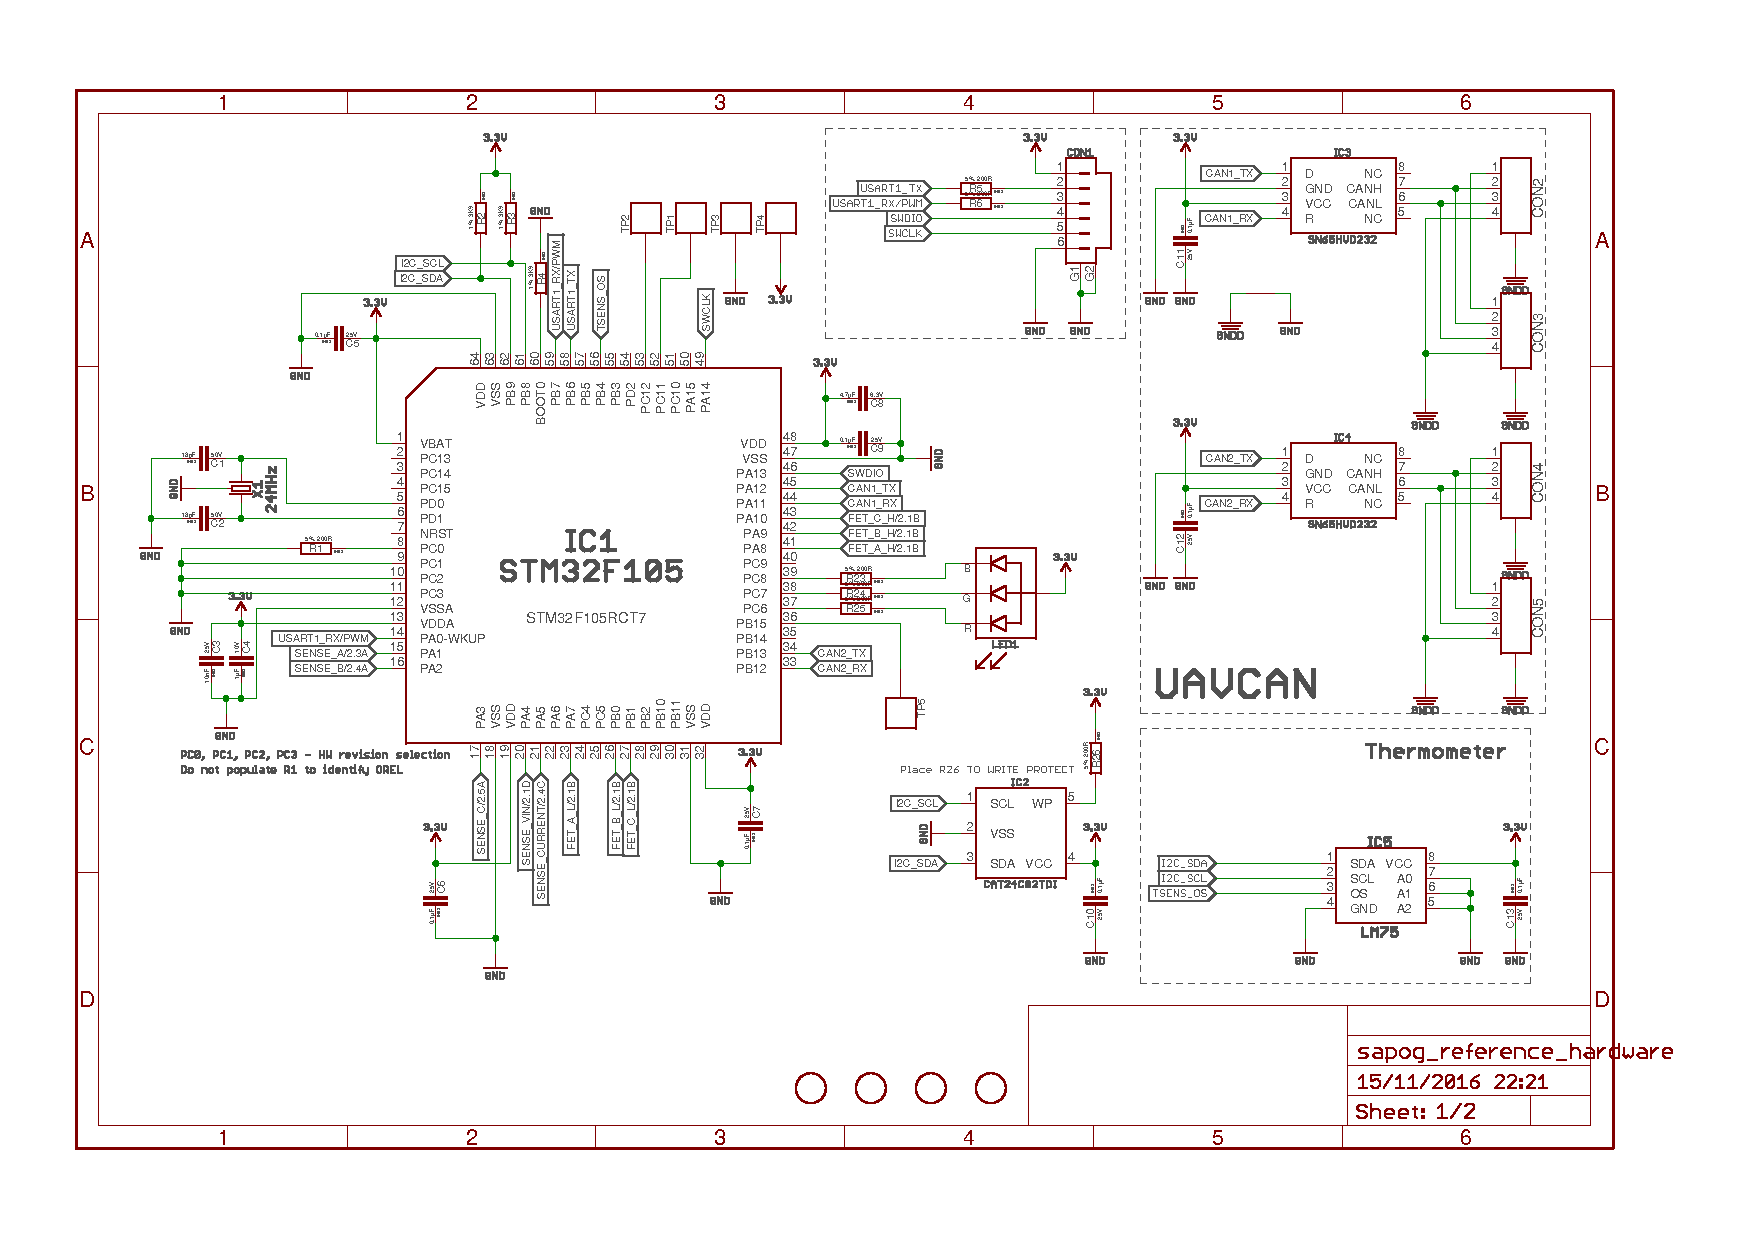
\includegraphics[page=1,angle=90,origin=c,width=1\textwidth]{sapog_reference_hardware.pdf}
	\caption{Reference schematic, page 1.}
\end{figure}

\begin{figure}[hbt]
    \centering
    \includegraphics[page=2,angle=90,origin=c,width=1\textwidth]{sapog_reference_hardware.pdf}
	\caption{Reference schematic, page 2.}
\end{figure}

\end{document}
